\documentclass[11pt]{article}
\usepackage{graphicx}
\usepackage{float}
\usepackage{amsmath}
\usepackage{amssymb}
\usepackage{dirtytalk} % For \say{}
\usepackage{caption}
\usepackage{subcaption}
\usepackage{hyperref}
\hypersetup{
    colorlinks=true,
    }

\setlength{\textwidth}{6.5in}
\setlength{\headheight}{0in}
\setlength{\textheight}{8.0in}
\setlength{\hoffset}{0in}
\setlength{\voffset}{0in}
\setlength{\oddsidemargin}{0in}
\setlength{\evensidemargin}{0in}

\def\dbar{{\mathchar'26\mkern-12mu d}}

\title{2D Ising Model Simulation}
\author{Salar Ghaderi, Xinyu Liu, Tongzhou Wang}
%alphabetic order

\date{December 2024}

\begin{document}

\maketitle

\abstract{We performed a Markov chain Monte Carlo algorithm to simulate the physic behavior of 2D Ising Model. First, we studied the model under static external magnetic field. We simulated the energy and magnetization when heating a two-dimensional square lattice Ising model. We start at absolute zero temperature with the system in both ground state and pseudo-ground state. We also performed a simulation for cooling the system initially above the critical temperature with random spin orientations. The simulation result at zero external magnetic field is compared with analytical prediction for an infinitely large system. We also discussed the effect of system size, $\mathbb{Z}_2$ symmetry, and the convergence issue of the Markov chain. Then, we briefly studied the system under nonstatic external field. In the appendix, we also tested the fluctuation of energy under our metropolis sampling.}

\section{Introduction}
\subsection{The Ising Model}
The Ising model is a theoretical model of ferromagnetism proposed by Ernst Ising in 1925 \cite{ising1925contribution, kramers1941statistics}. In the two-dimensional square lattice Ising model, a magnetic material is modeled by a two-dimensional square lattice with magnetic dipoles (due to the spins of the particles) on the lattice sites. The magnetic dipoles are assumed to be capable of pointing in only two directions, up or down, characterized by $s = \pm 1$. It is further assumed that a magnetic dipole interacts only with its four nearest neighbors (for dipoles on the edges, periodic boundary conditions are assumed). Thus, the total energy of the system is given by
\begin{equation}\label{Hamiltonian}
    E = -J \sum_{\langle ij \rangle} s_i s_j - H \sum_{i} s_i,
\end{equation}
where $J$ is a positive interaction constant and $H$ accounts for an external magnetic field. The notation $\langle ij \rangle$ indicates a sum over pairs $s_i$, $s_j$ that are adjacent on the lattice.

For a system of $N \times N$ dipoles, the magnetization (magnetic dipole moment density) can be characterized by
\begin{equation}\label{magnetization}
    M = \frac{1}{N^2}\sum_{i} s_i.
\end{equation}
For the special case of $H = 0$ and an infinitely large system($N \rightarrow +\infty$), there is an analytical expression of the magnetization as a function of temperature
\begin{equation}\label{theoryM}
    M(T) = \begin{cases}
            0, & T > T_c, \\
            \frac{(1 + z^2)^{1/4} (1 - 6z^2 + z^4)^{1/8}}{\sqrt{1-z^2}}, & T < T_c,
    \end{cases}
\end{equation}
where $kT_c / J \approx 2.269185$ is the critical temperature, $z = \exp(-2J/kT)$, and $k$ is the Boltzmann constant. This analytical solution of the 2D square lattice Ising model was derived by Lars Onsager in 1944 \cite{onsager1944crystal}. For the general case $H \neq 0$, an analytical solution has not been found yet. In the following chapter, We will provide simulation result for the behavior of $H$ and $E$ with $T$ at both heating and cooling. The simulation under zero external magnetic field $H$ will be compared with this an analytical prediction.

\subsection{Expected Behaviors at High and Low Temperatures}
In the absence of a magnetic field, it is expected that at sufficiently high $T$, $M \sim 0$, and at sufficiently low $T$, $M \sim \pm 1$. This can be understood from two perspectives.

From a physics perspective, during any isothermal and isobaric processes, a system's change in its Gibbs free energy satisfies $dG \leq 0$, where the equality only holds for reversible processes, which are unrealistic idealizations. For isothermal processes we have $dG = d\mathcal{H} - TdS$, where $\mathcal{H}$ is the enthalpy and $S$ is the entropy.

At high $T$, $dG$ is dominated by $-TdS$, so the system must change in a way such that $dS > 0$. For our system, $S$ is maximized when there is an equal amount of spins in both directions, so $M = (1/N^2) \sum_i s_i \sim 0$.

At low $T$, $dG$ is dominated by $d\mathcal{H}$, so the system must change in a way such that $d\mathcal{H} < 0$. For our system, the energy is the lowest when all spins are aligned because $E = -J \sum_{\langle ij \rangle} s_i s_j$. Therefore, $M = (1/N^2) \sum_i s_i \sim \pm 1$.

From an algorithmic perspective, in the Metropolis algorithm, we accept the move with acceptance probability ((10.60) in Newman \cite{newman2013computational})
\begin{equation}\label{acceptprob}
    P_a = \begin{cases}
        1, & \Delta E \leq 0, \\
        e^{-\beta \Delta E}, & \Delta E > 0.
    \end{cases}
\end{equation}

At high $T$, $\beta \rightarrow 0$, (\ref{acceptprob}) becomes
\begin{equation}
    P_a \approx \begin{cases}
        1, & \Delta E \leq 0, \\
        1, & \Delta E > 0.
    \end{cases}
\end{equation}
This means that the move will be accepted no matter it decreases the energy (aligns more spins) or increases the energy (reverses more spins). The upshot will be an equal amount of spins in both directions, so $M = (1/N^2) \sum_i s_i \sim 0$.

At low $T$, $\beta \rightarrow \infty$, (\ref{acceptprob}) becomes
\begin{equation}
    P_a \approx \begin{cases}
        1, & \Delta E \leq 0, \\
        0, & \Delta E > 0.
    \end{cases}
\end{equation}
This means that the move will be accepted only if it decreases the energy (aligns more spins) or does not change the energy. The upshot will be that all spins are aligned, so $M = (1/N^2) \sum_i s_i \sim \pm 1$. Thus, the Metropolis algorithm agrees with the physical argument. In fact, in this case the Metropolis algorithm simulates the random flipping of spins due to thermal fluctuation.

\subsection{Summary of Main Results}
In Section \ref{method}, we explain our rescaling of variables, the Markov chain, the Metropolis algorithm, the periodic boundary condition and the software and physical setup for our system. In Section \ref{result1}, we present our main result and discussions under static external field. We find that under zero external field, the simulation agrees with the analytical result. We also discussed the effect of system size and the $\mathbb{Z}_2$ symmetry of the theory. We found that the $\mathbb{Z}_2$ symmetry is conserved in our simulation. We observe the occurrence of global spin flipping when heating the metastable ground state from zero temperature and we propose that it's from the convergence issue. We prove our proposal with data. The simulation for cooling the system under zero external field also agrees with the analytical result. In Section \ref{result2}, we study the system under non-uniform spatial external field. In the Appendix \ref{appendix}, we delve deeper to look into the fluctuation of energy$\langle \Delta E^2 \rangle$. 
% Since the fluctuation-dissipation theorem is a property of thermal ensemble, our result provide evidence to the success of converging and generating a thermal ensemble in the metropolis algorithm.

\section{Method}\label{method}

\subsection{Rescaling the Variables}

Since we're carrying out numerical simulations, we first redefine all physical quantities in a dimensionless way. The rescaled energy is:

\begin{equation}
    E' = E / J
\end{equation}

The rescaled external magnetic field is:

\begin{equation}
    H' = H / J
\end{equation}

The total energy is thus:

\begin{equation}
    E' = -\sum_{\langle ij \rangle} s_i s_j - H' \sum_{i} s_i,
\end{equation}

At the same time, the temperature is rescaled by:

\begin{equation}
    T' = kT/J
\end{equation}

Where $k$ is the Boltzmann constant. This dimensionless temperature denotes relative scale of thermal fluctuation and internal energy. With this dimensionless temperature $T'$, external magnetic field $H'$ and energy $E'$, we can carry out the further numerical simulation.

\subsection{Markov Chain Monte Carlo Simulation}
We perform a Markov chain Monte Carlo simulation with the Metropolis algorithm to find the energy and magnetization of a 2D square lattice Ising model.

The fundamental problem in statistical mechanics is to calculate the expectation value of a quantity of interest for a system in thermal equilibrium at temperature $T$
\begin{equation}\label{exp}
    \langle X \rangle = \sum_i X_i P(E_i),
\end{equation}
where $P(E_i)$ is given by the Boltzmann distribution
\begin{equation}
\begin{gathered}
    P(E_i) = \frac{e^{-\beta E_i}}{Z} \quad \text{with} \quad Z = \sum_i e^{-\beta E_i}.
\end{gathered}
\end{equation}
In our case, the quantities of interest are the energy and magnetization of the 2D square lattice Ising model.

The expectation value $\langle X \rangle$ in (\ref{exp}) can be estimated by randomly choosing $N$ states according to the Boltzmann distribution and taking the average of their $X_k$, that is
\begin{equation}\label{estimate}
    \langle X \rangle \approx \frac{1}{N} \sum_{k=1}^{N} X_k.
\end{equation}
However, selecting states according to the Boltzmann distribution is nontrivial, and is accomplished with the Markov chain.

\subsubsection{The Markov chain}

We want to choose a set of states for the sum (\ref{estimate}). We will do so by generating a chain of states one after another\textemdash the Markov chain. The choice of the next state following the previous state is determined by a set of transition probabilities $T_{ij}$ that give the probability of changing from state $i$ to state $j$. It is required that $\sum_j T_{ij} = 1$. 

If we further require the transition probabilities $T_{ij}$ to satisfy
\begin{equation}\label{cond}
    \frac{T_{ij}}{T_{ji}} = \frac{P(E_j)}{P(E_i)} = \frac{e^{-\beta E_j} / Z}{e^{-\beta E_i} / Z} = e^{-\beta (E_j - E_i)},
\end{equation}
then it can be proved that if you start off the system in any random state and run the Markov chain for long enough, the distribution over states will converge to the Boltzmann distribution \cite{newman2013computational}.

\subsubsection{The Metropolis Algorithm}
We still need to choose the transitional probabilities $T_{ij}$ so that they satisfy (\ref{cond}). The most common way to do this is using the Metropolis algorithm, which works as follows.

For a state in the Markov chain, we choose the next state uniformly at random from a specified set of possible states, called a move set. Then, we either accept or reject the new state with acceptance probability $P_a$ given by
\begin{equation}\label{acceptprob}
    P_a = \begin{cases}
        1, & \Delta E \leq 0, \\
        e^{-\beta \Delta E}, & \Delta E > 0.
    \end{cases}
\end{equation}
If the new state is accepted, then we move the system from the old state to the new state. If the new state is rejected, then we move the system from the old state to the old state itself (i.e. the system remains in its old state for one more step). 

We can prove that with the Metropolis algorithm, the transition probabilities $T_{ij}$ satisfy (\ref{cond}). We suppose that the move sets of state $i$ and state $j$ both contain $M$ states. If $E_j > E_i$, then
\begin{equation}
    T_{ij} = \frac{1}{M} e^{-\beta (E_j - E_i)} \quad \text{and} \quad T_{ji} = \frac{1}{M},
\end{equation}
and the ratio of the two is
\begin{equation}
    \frac{T_{ij}}{T_{ji}} = e^{-\beta (E_j - E_i)}.
\end{equation}
Conversely, if $E_i \geq E_j$, then
\begin{equation}
    T_{ij} = \frac{1}{M} \quad \text{and} \quad T_{ji} = \frac{1}{M} e^{-\beta (E_i - E_j)},
\end{equation}
and the ratio of the two is again
\begin{equation}
    \frac{T_{ij}}{T_{ji}} = e^{-\beta (E_j - E_i)}.
\end{equation}
Either way, (\ref{cond}) is satisfied.

To summarize, the Markov chain Monte Carlo simulation with the Metropolis algorithm involves the following steps:
\begin{enumerate}
    \item Choose the starting state, which can be any state of the system.
    \item Choose the next state uniformly at random from the move set.
    \item Compute the acceptance probability $P_a$ given by (\ref{acceptprob}), and accept or reject the new state accordingly.
    \item Compute and record the quantity of interest in the current state.
    \item Repeat from step 2.
\end{enumerate}
After the distribution of states in the Markov chain converges to the Boltzmann distribution, we can start estimating the expectation of the quantity of interest according to (\ref{estimate}). One can often tell whether the convergence has occurred just by observing the quantity of interest of the states in the Markov chain.

\subsection{Periodic Boundary Conditions}

With limited computational resources, we cannot perform a calculation on an infinitely large system. In order to minimize the effect from the finiteness of our system, we perform our simulation using periodic boundary condition. In our simulation, the $N^{th}$ atom interact with the $1^{st}$ atom on both columns and rows, such that we're effectively simulating an infinitely large system while assuming periodicity.

\subsection{Physical and Software Setup}

Here we briefly discuss our software setup. In most of our results, we choose a $500*500$ 2D system. We also vary the magnetization $H'$ in a fixed set($H' = \pm 0.5,\pm0.1,0$). We start our simulation by increasing our temperature from zero \ref{heating} \label{heating} and decreasing temperature \ref{cooling}. For each temperature, we perform a metropolis algorithm to simulate a thermal ensemble. We have an iteration size which denotes the size of Markov chain. Without specific notification, we always use the last 10\% of the chain as our ensemble to calculate the energy and magnetization of the system, assuming that the system has converged to equilibrium.

In order to know how many iteration steps are required for our model to converge, we perform some pre-simulation at certain different temperatures. We plot the magnetization and energy of our model during iteration, and thus we can directly see whether the energy becomes stable in the Markov chain. We find that the required iteration is much larger near phase transition. This is quite intuitive: when the temperature change in each step is fixed, the model is expected to have much larger changes near the phase transition, and this requires more iteration to stabilize. In our script, without special specification, we set the iteration near phase transition to be $2*10^8$. At different temperature, the iteration step is less than $6*10^6$. We find that this set up can lead to stabilization at different temperature as well as saving computing resource.

 
% We will show that, the ensemble we have simulated is not only close to a thermal ensemble in the sense of energy expectation$\langle E \rangle$, but also in the sense of energy fluctuation$\langle \Delta E^2 \rangle$.



\section{Result on External Magnetic Field}\label{result1}

The Ising model system has two stable states under zero temperature. With the existence of a uniform external magnetic field, the true ground state has all spins align with the external field. There also exists a pseudo ground state or metastable state whose spins anti-align with the external field. Although this metastable state does not have the lowest energy, any local disturbance(single spin flipping) increases the energy(when the external field $H'$ is not extremely strong). When we start to heat up the system from zero temperature, choosing true ground state and pseudo ground state lead to different behavior. We are interested in both two scenarios. Also, we present our simulation on cooling from a high temperature.


\subsection{Heating from True Ground State}\label{heating}

The source codes for this part can be found at: \url{https://github.com/rising1227/phys-ga2000/tree/main/2DIsingModel1}

\subsubsection{Main Results}

We have simulated the relation between $M$ and $E'$ and $T'$ and plotted the figure as follows\ref{ET500here},\ref{MT500here}. In each diagram we have simulated the behavior of a 500*500 2D Ising model when heating from absolute zero temperature and a true ground state. The iteration step number for the $H'=0$ case at $2.1 < T' < 2.5$ is $2*10^8$. The iteration step number is $2*10^5$ for $T' < 1.2$ and for all other cases, the iteration number is $8*10^6$. 

The diagram \ref{MT500here} shows the magnetization $M$ as a function of $T'$. For the zero external magnetization case, our simulation data is close to the analytical prediction for infinitely large system. With or without an external magnetic field, The magnetization $|M|$ of the system is generally weaker when the temperature is increased. However, the decrease of $|M|$ along $T'$ is sharper and faster when the external field $H'$ is weak and it's smoother when $H'$ is large. For very low temperature $T' < 1$, the system always stays at full magnetization $|M| = 1$ for all external field.

The diagram \ref{ET500here} shows the system energy $E'$ as a function of $T'$. Since we find that inverting the external field almost keep $E'-T'$ curve unchanged(we will discuss more about this symmetry in next chapter \ref{Z2}), here we only show our result for positive external field. The system energy exhibit to stay almost remains unchanged at low temperature $T'<1$, which shows that the system almost always stays at a true ferromagnetic state when the temperature is low. When the system approaches the critical temperature $T_C$, the energy shows accelerating growth with increasing $T'$. When the temperature becomes higher than around $T'=3$ the growth starts to decelerate. The growing trend $E'-T'$ is sharper and steeper for the zero external field case.

\begin{figure}
    \centering
    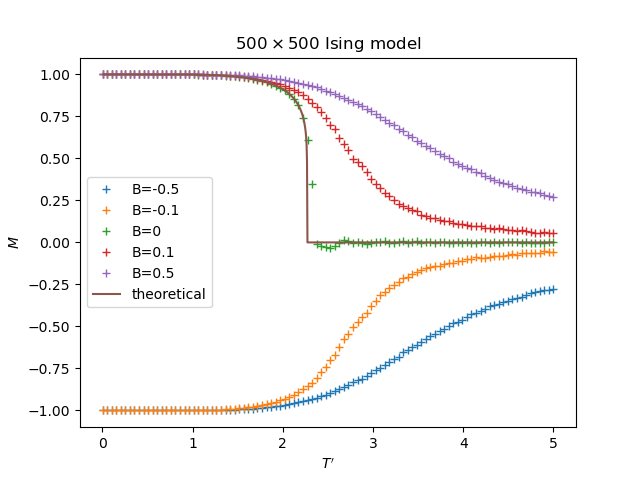
\includegraphics[width=0.6\linewidth]{plots/M-T_withB_diagram(latest,500).png}
    \caption{$M$-$T'$ relation for N=500 2D Ising model}
    \label{MT500here}
\end{figure}

\begin{figure}
    \centering
    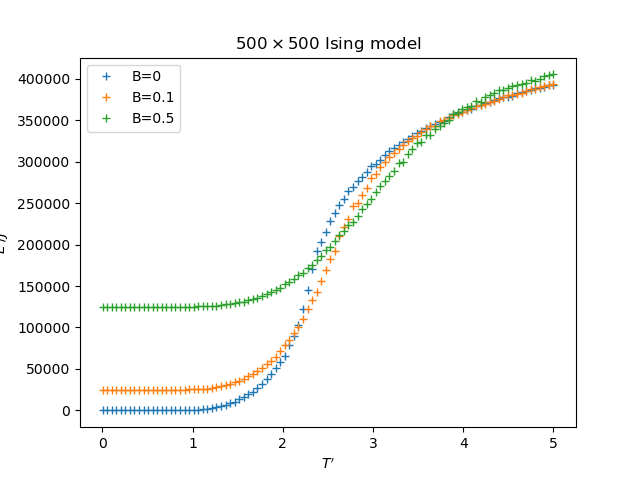
\includegraphics[width=0.6\linewidth]{plots/E-T_withB_diagram(latest,500).png}
    \caption{$E'$-$T'$ relation for N=500 2D Ising model}
    \label{ET500here}
\end{figure}

\subsubsection{Discussion on System Size}

After simulating a system with $N=500$, we further investigate how does the system size affect the simulation. Our motivation is that the analytical result of magnetization over temperature\ref{theoryM} only holds for an infinitely large system ($N \rightarrow +\infty$). We investigate how the finiteness of our system affect the simulation outcome. We do the simulation for 3 different $N$(100,200,300) and compare the $E'-T'$\ref{E-T/N} and $M-T'$\ref{M-T/N} relation.

We find that the general simulation result between energy, magnetization and temperature appears to be the same for different system size. However, the significant difference is that for larger system the fluctuation of $E'$ and $M$ is larger. The curve of $E'-T'$ and $M-T'$ is smoother for larger system.\label{smoothdiscussion} We'll delve deeper into this phenomena in the appendix\ref{appendix} when we look at testing the fluctuation-dissipation theorem.

We also find that the $H'=0$ simulation result fits well with the analytical prediction for all different size(N=100,200 and 300). This is presented in the following diagram\ref{noH}. This indicates that although a well-defined phase transition is only happening at a infinitely large system, we can already observe a sharp phase-transition-like behavior starting from a system with $O(10^4)$ spins.


\begin{figure}
    \centering
    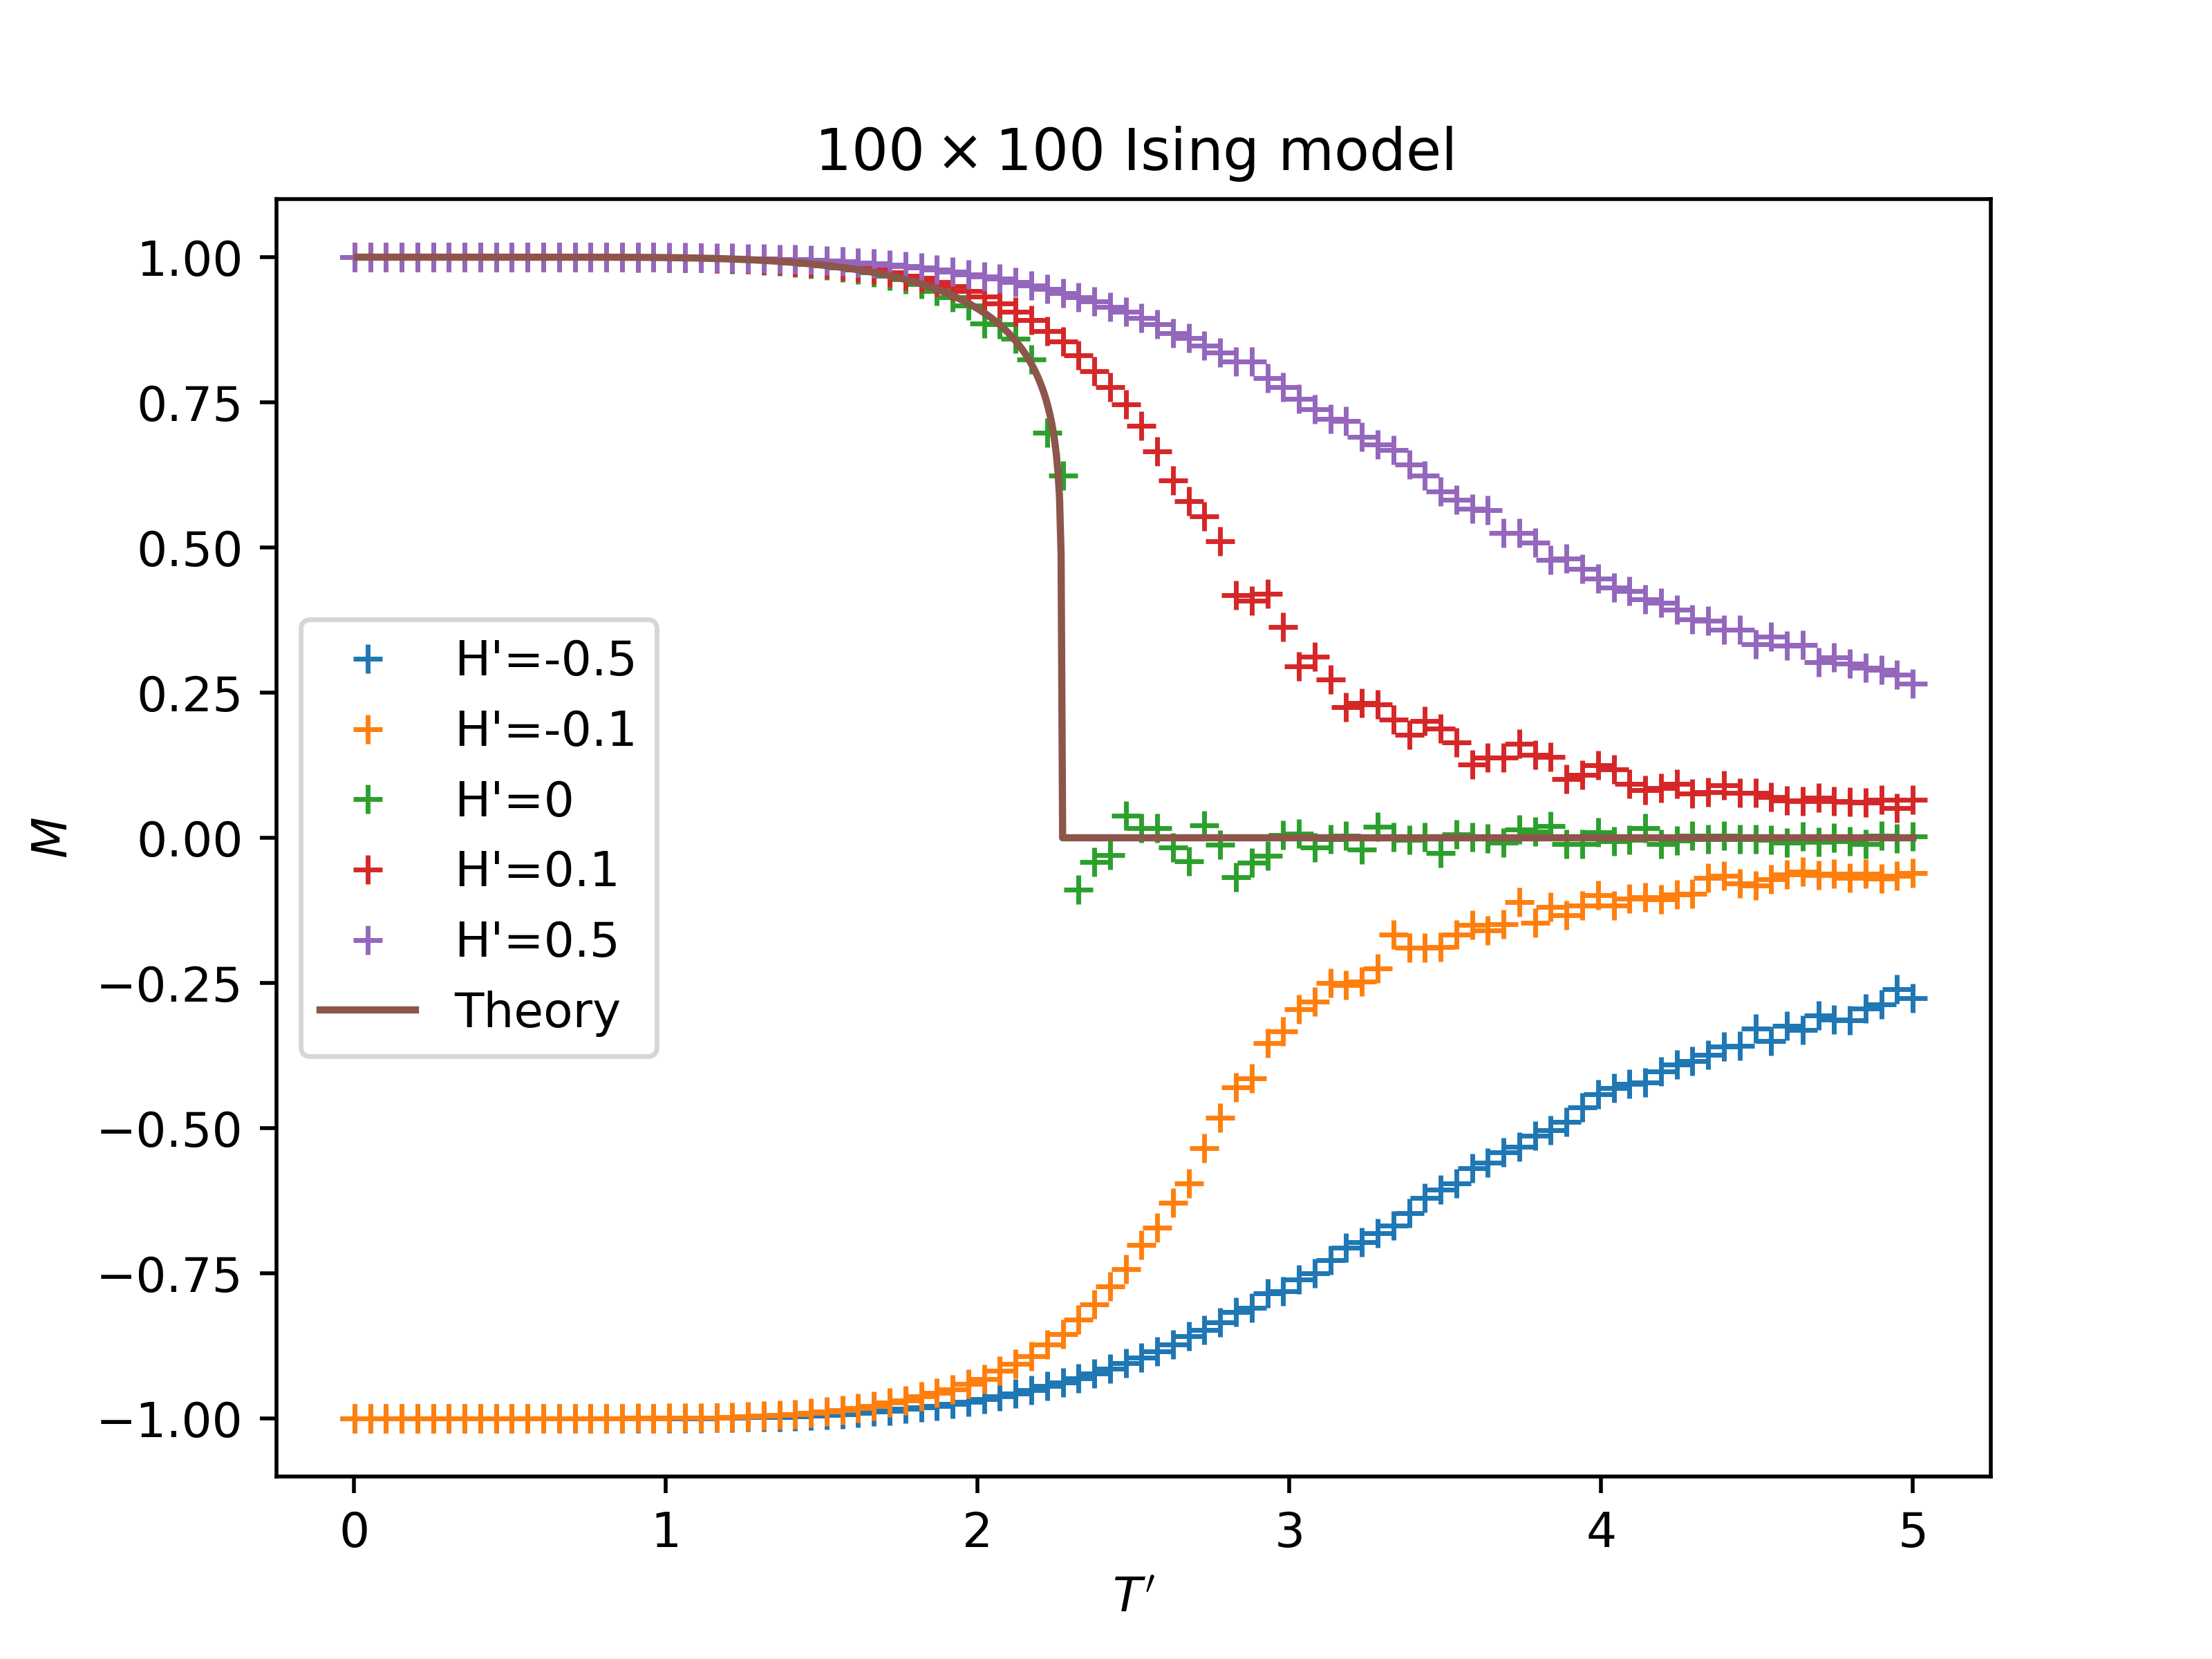
\includegraphics[width=0.48\textwidth]{plots/M-T_withB_diagram(latest,100).png}\hfill
    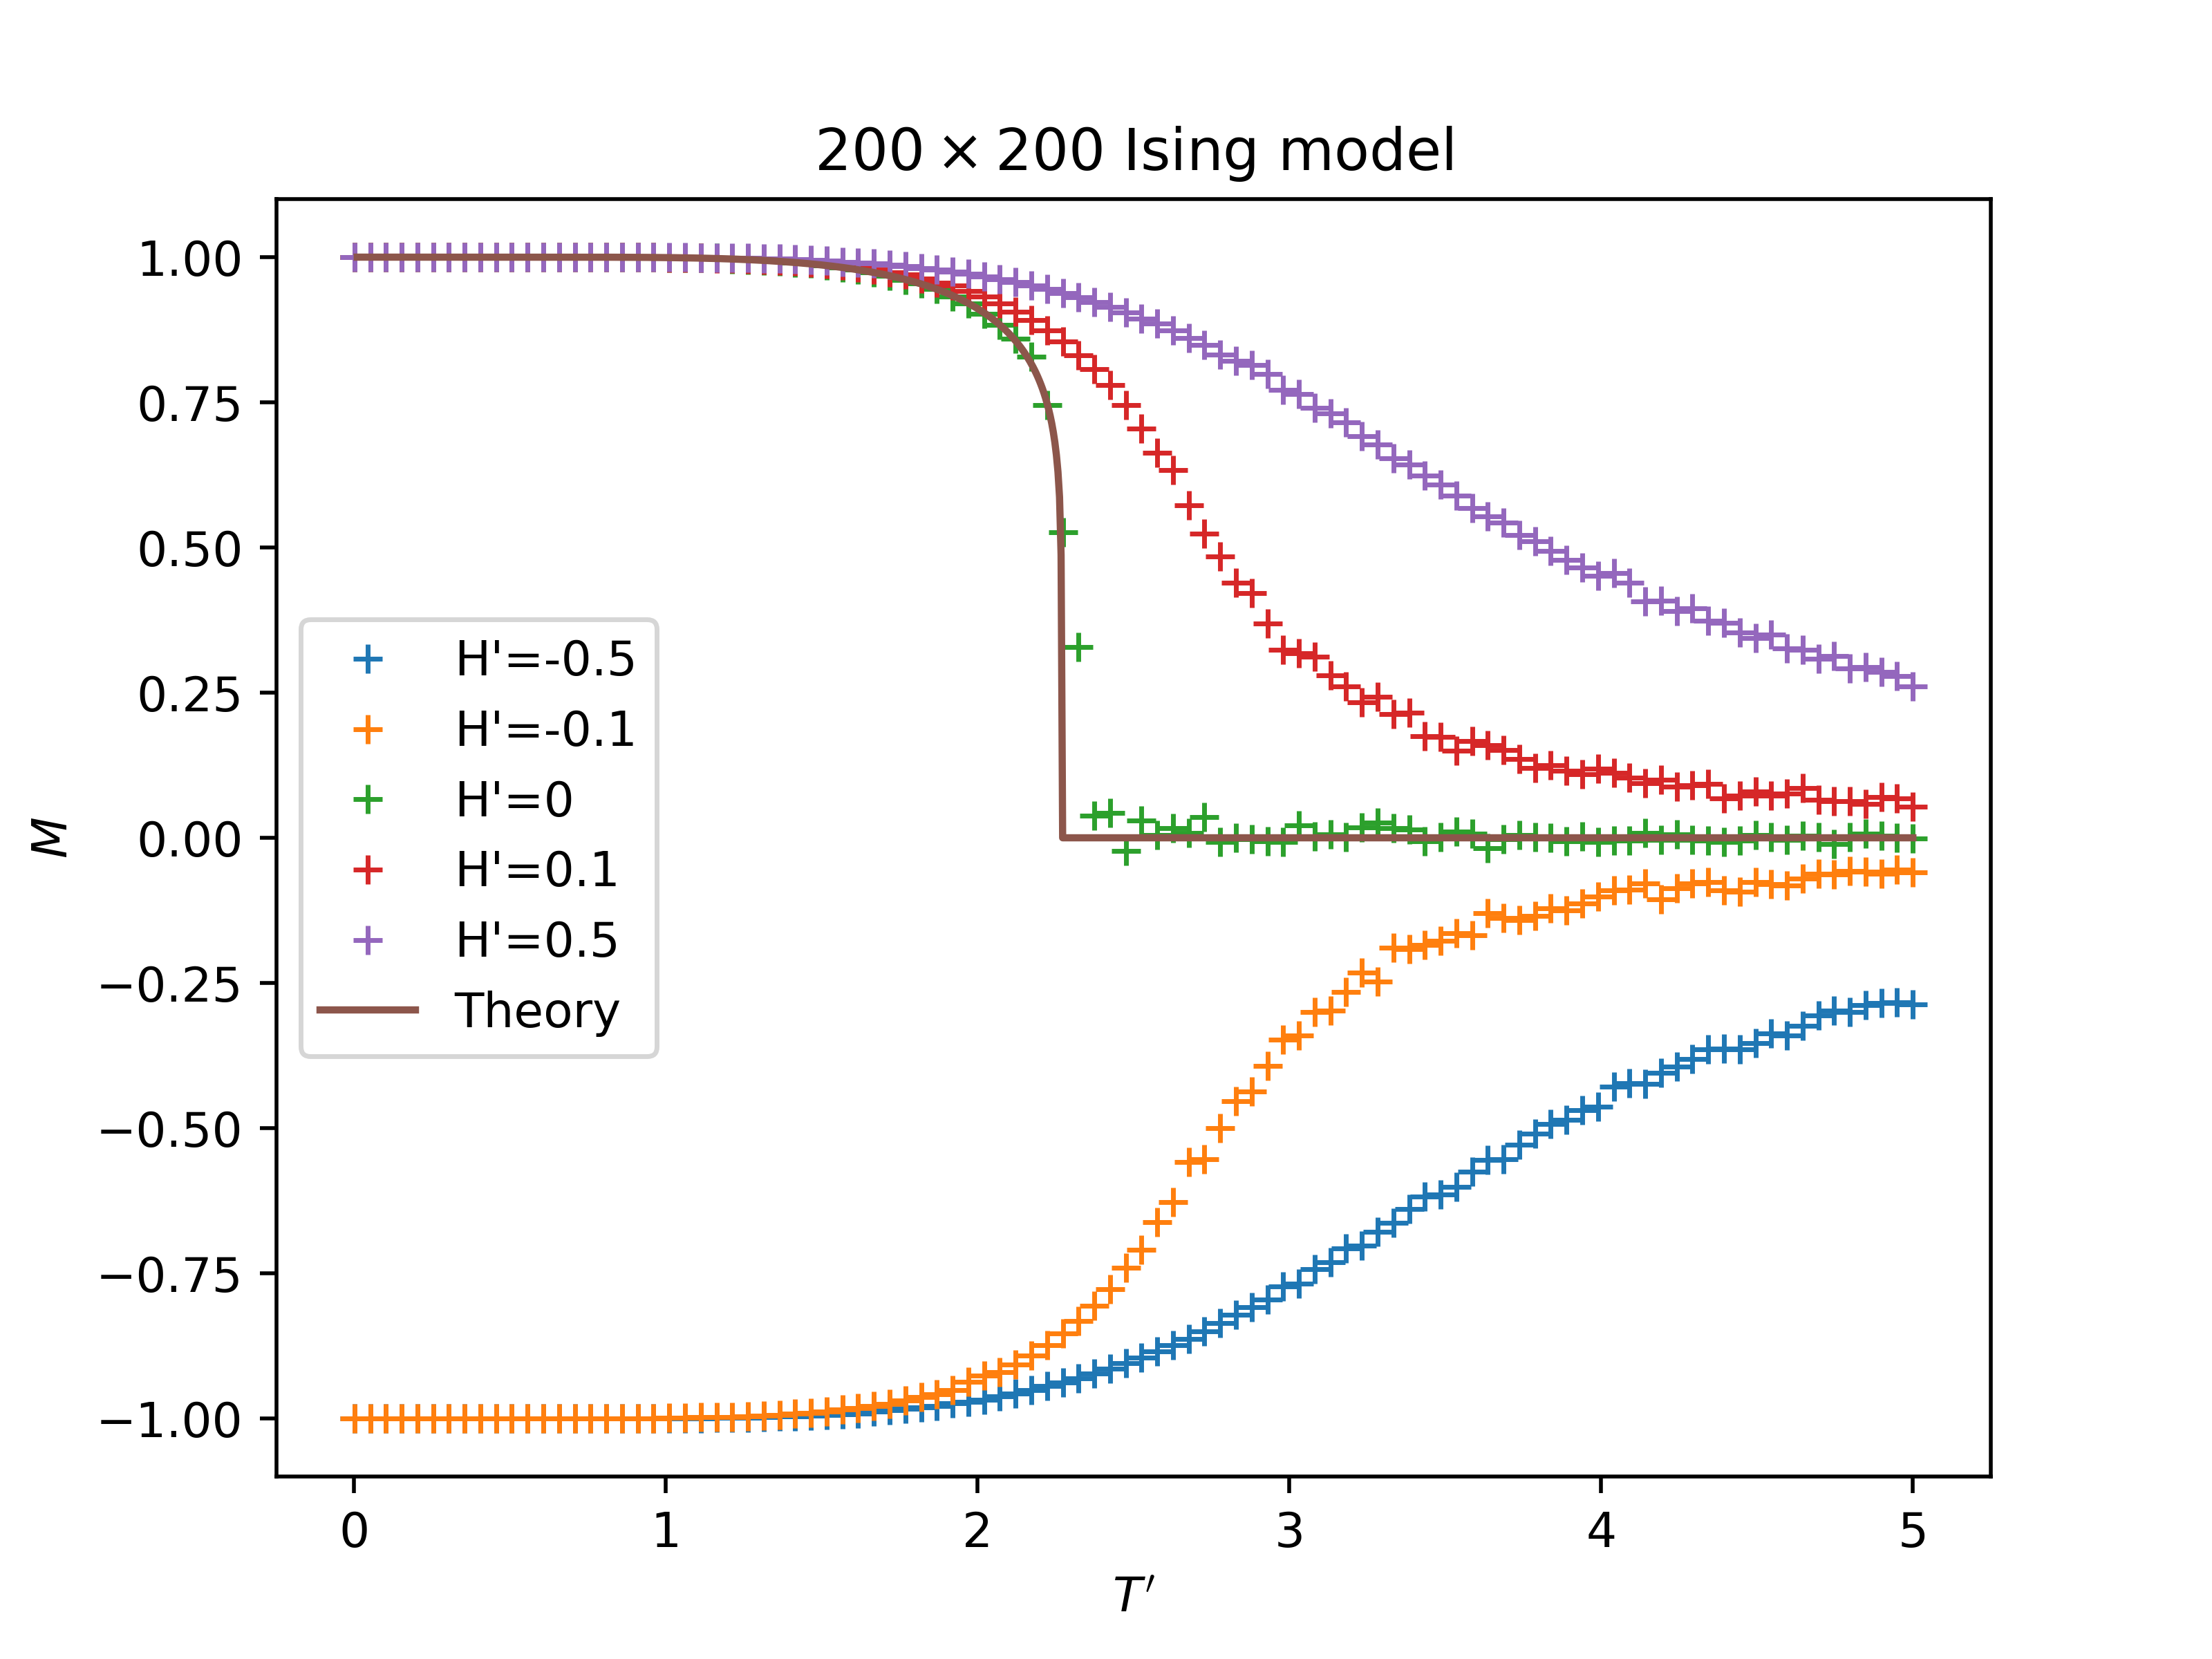
\includegraphics[width=0.48\textwidth]{plots/M-T_withB_diagram(latest,200).png}\hfill
    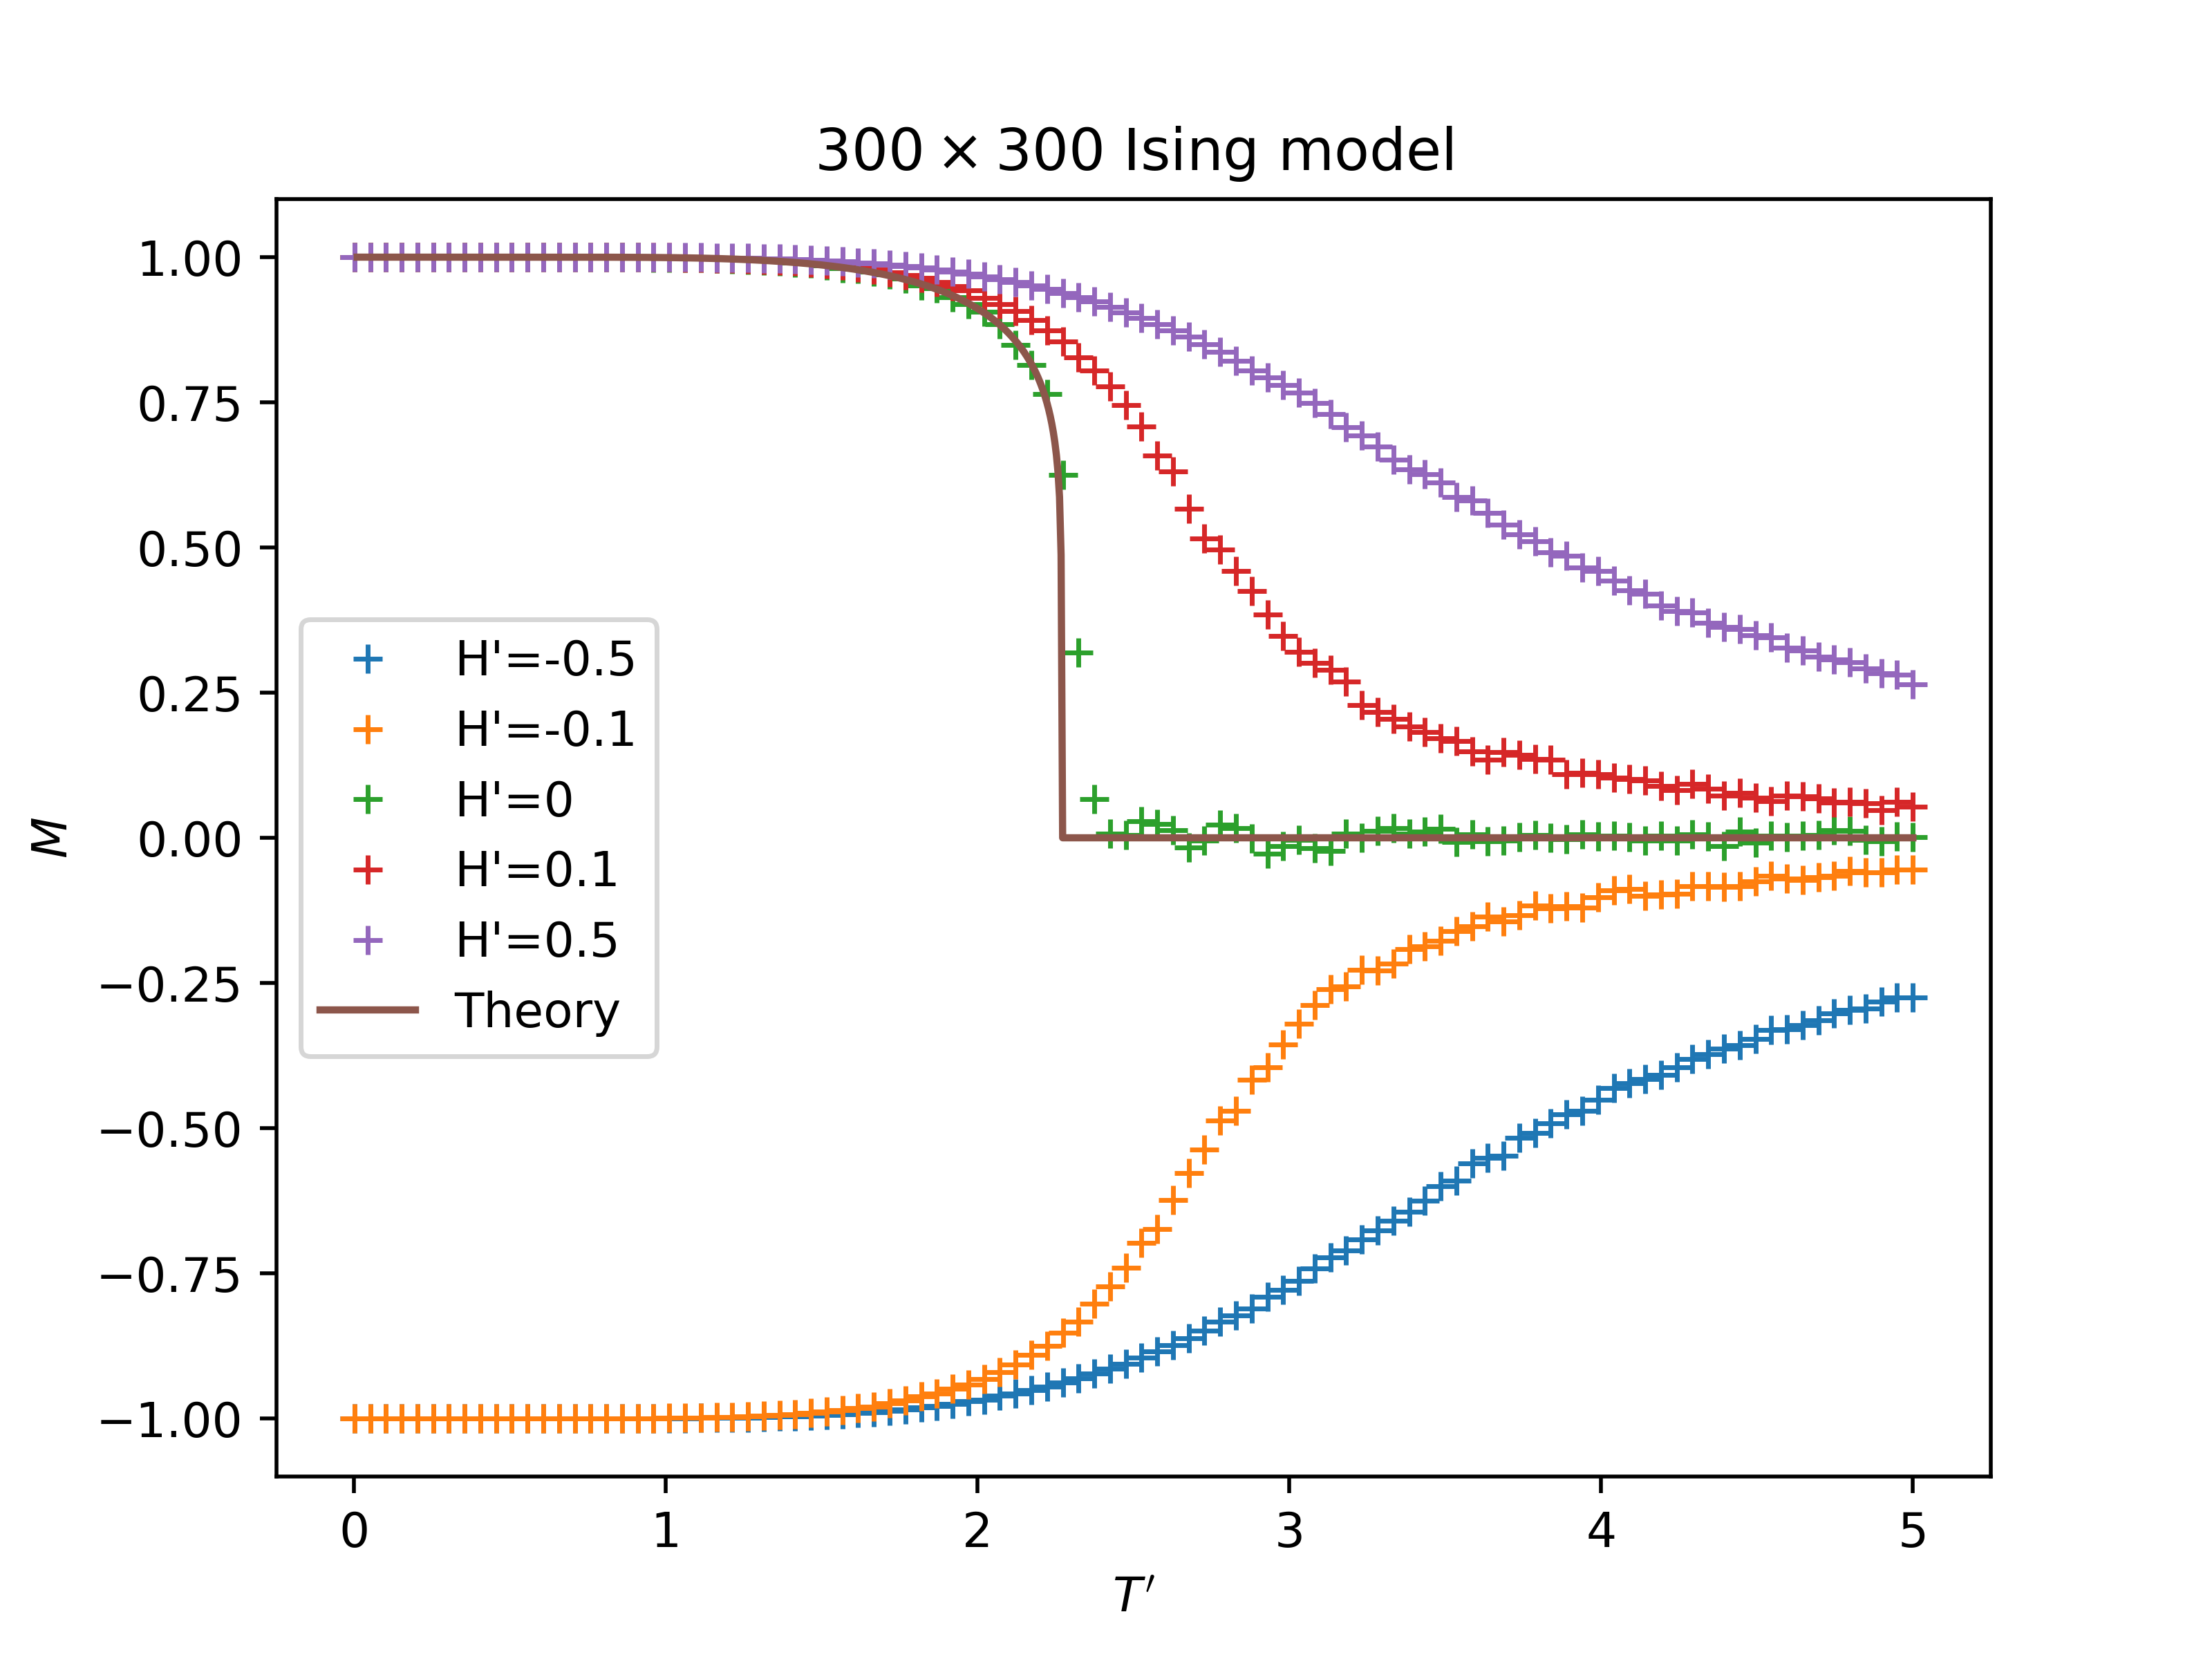
\includegraphics[width=0.48\textwidth]{plots/M-T_withB_diagram(latest,300).png}
    \caption{$M-T'$ relation of different system size $N$}
    \label{M-T/N}
\end{figure}

\begin{figure}
    \centering
    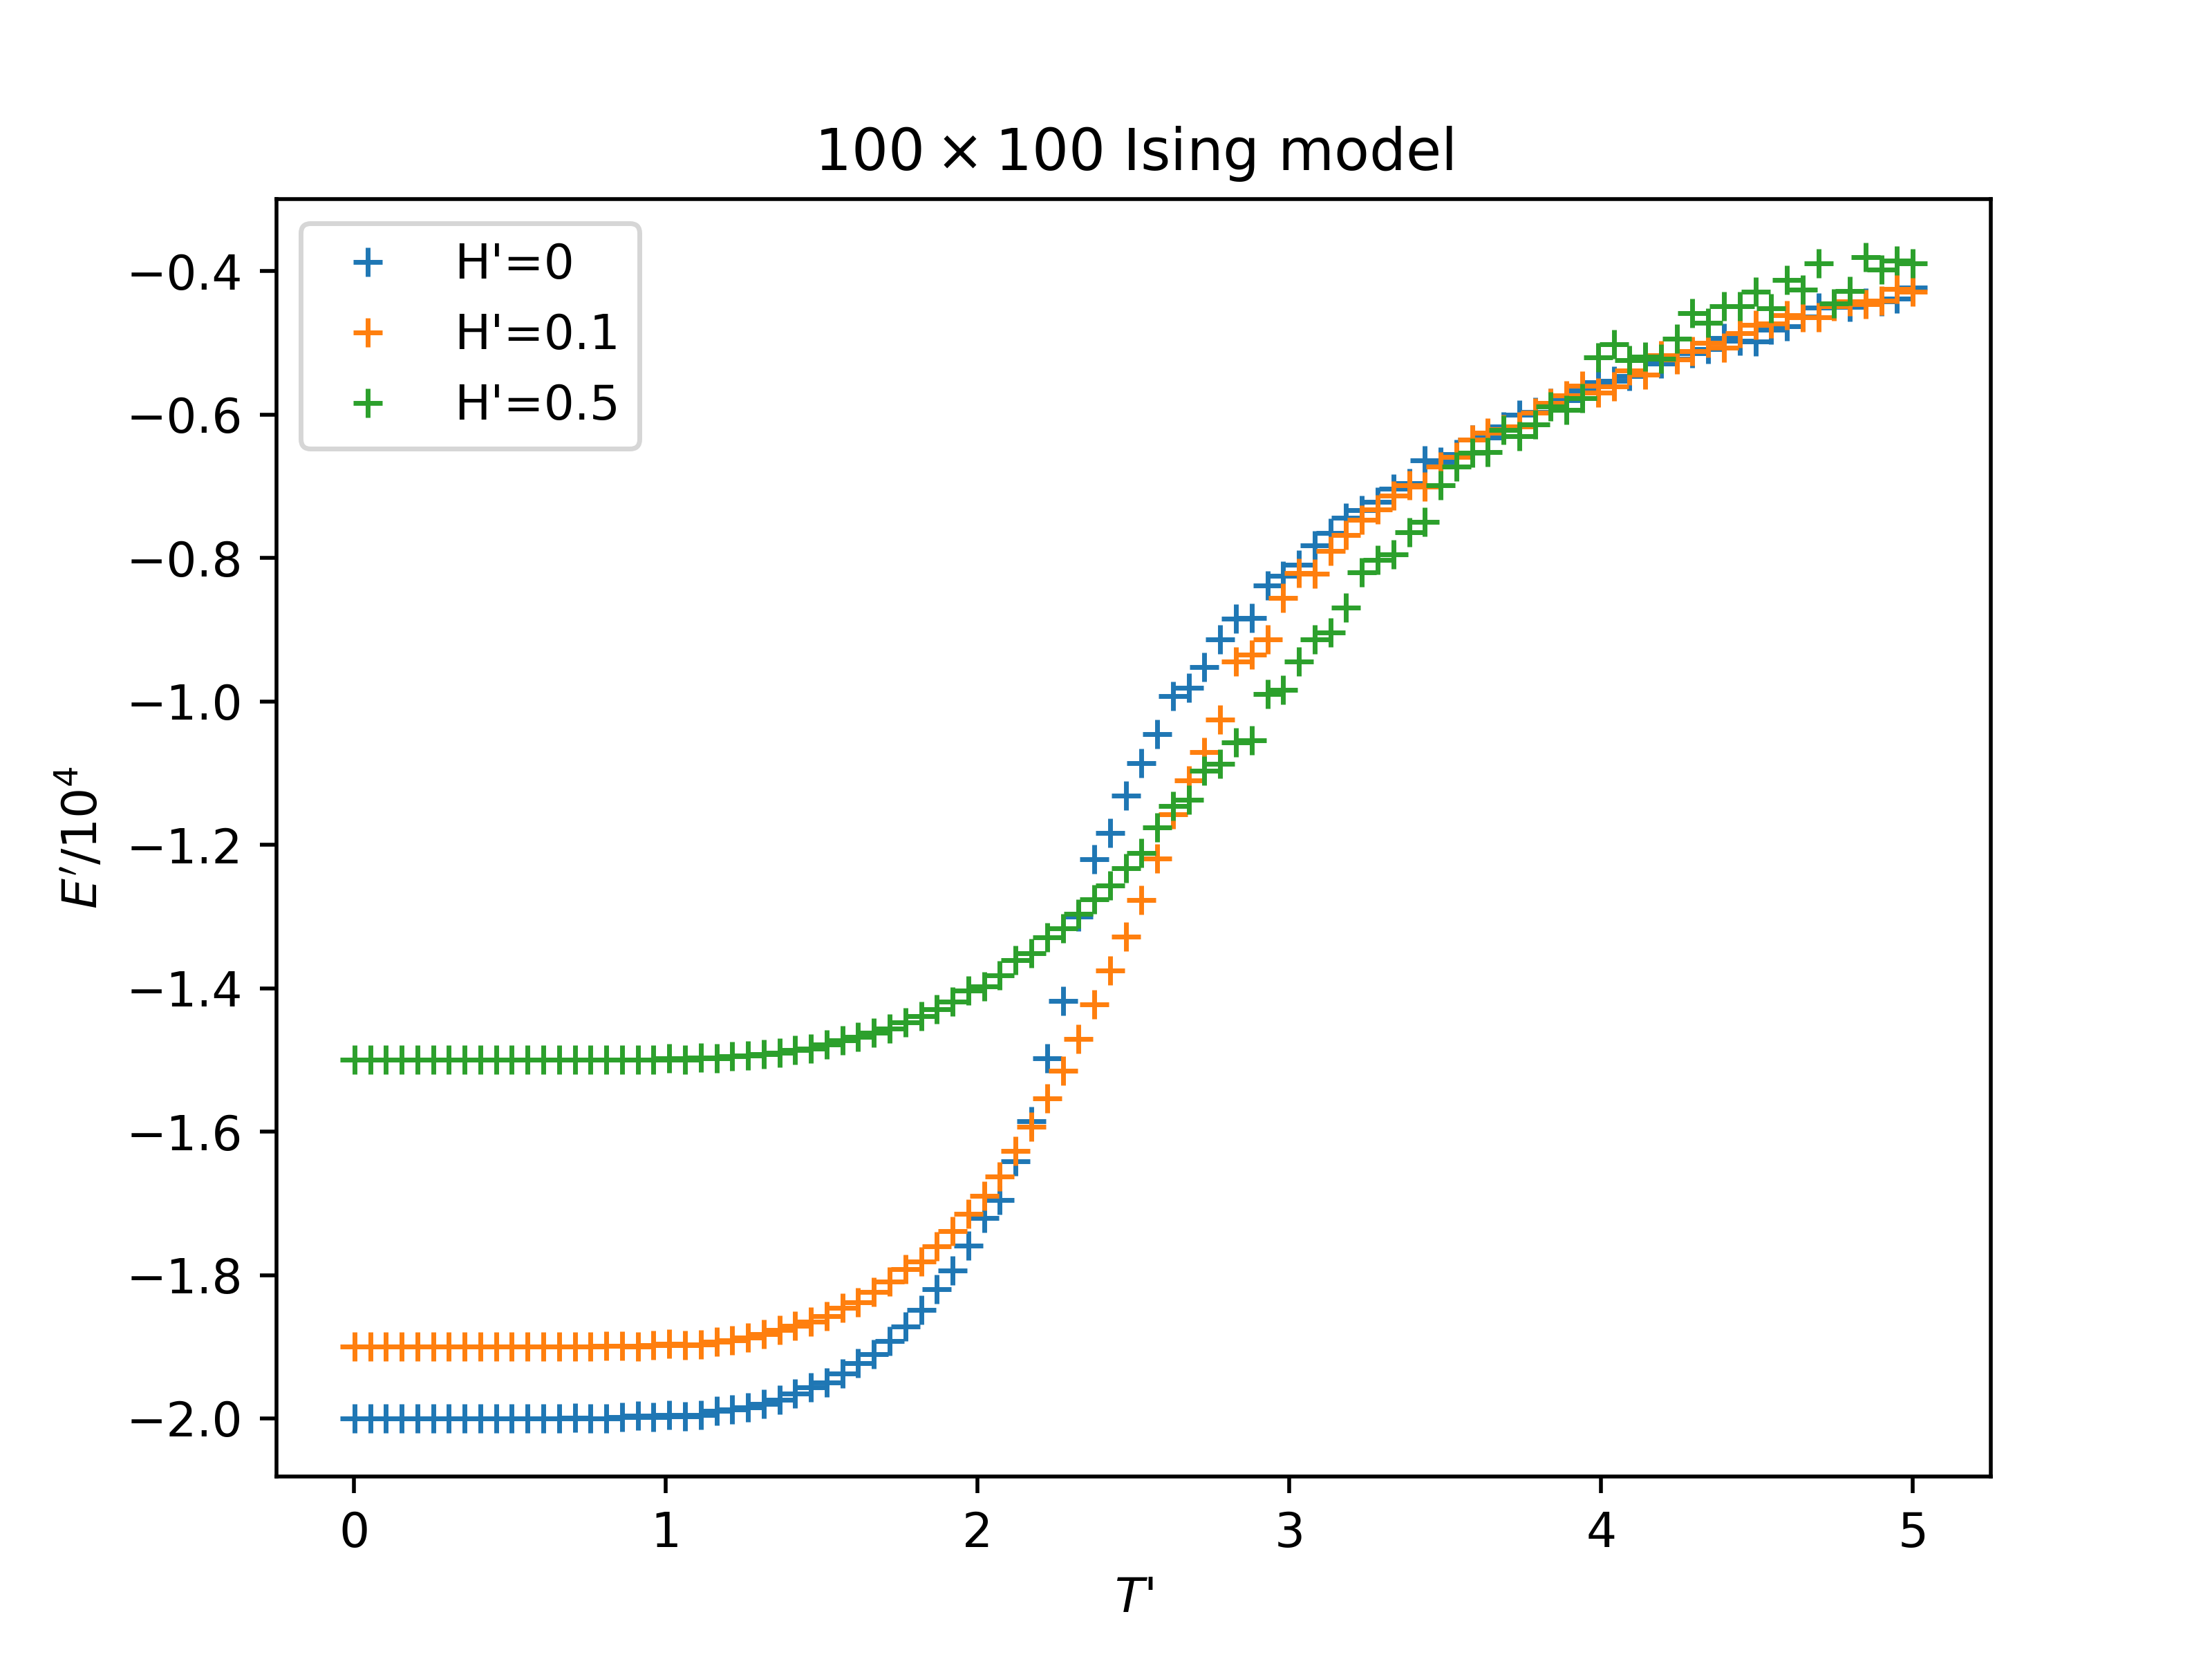
\includegraphics[width=0.48\textwidth]{plots/E-T_withB_diagram(latest,100).png}\hfill
    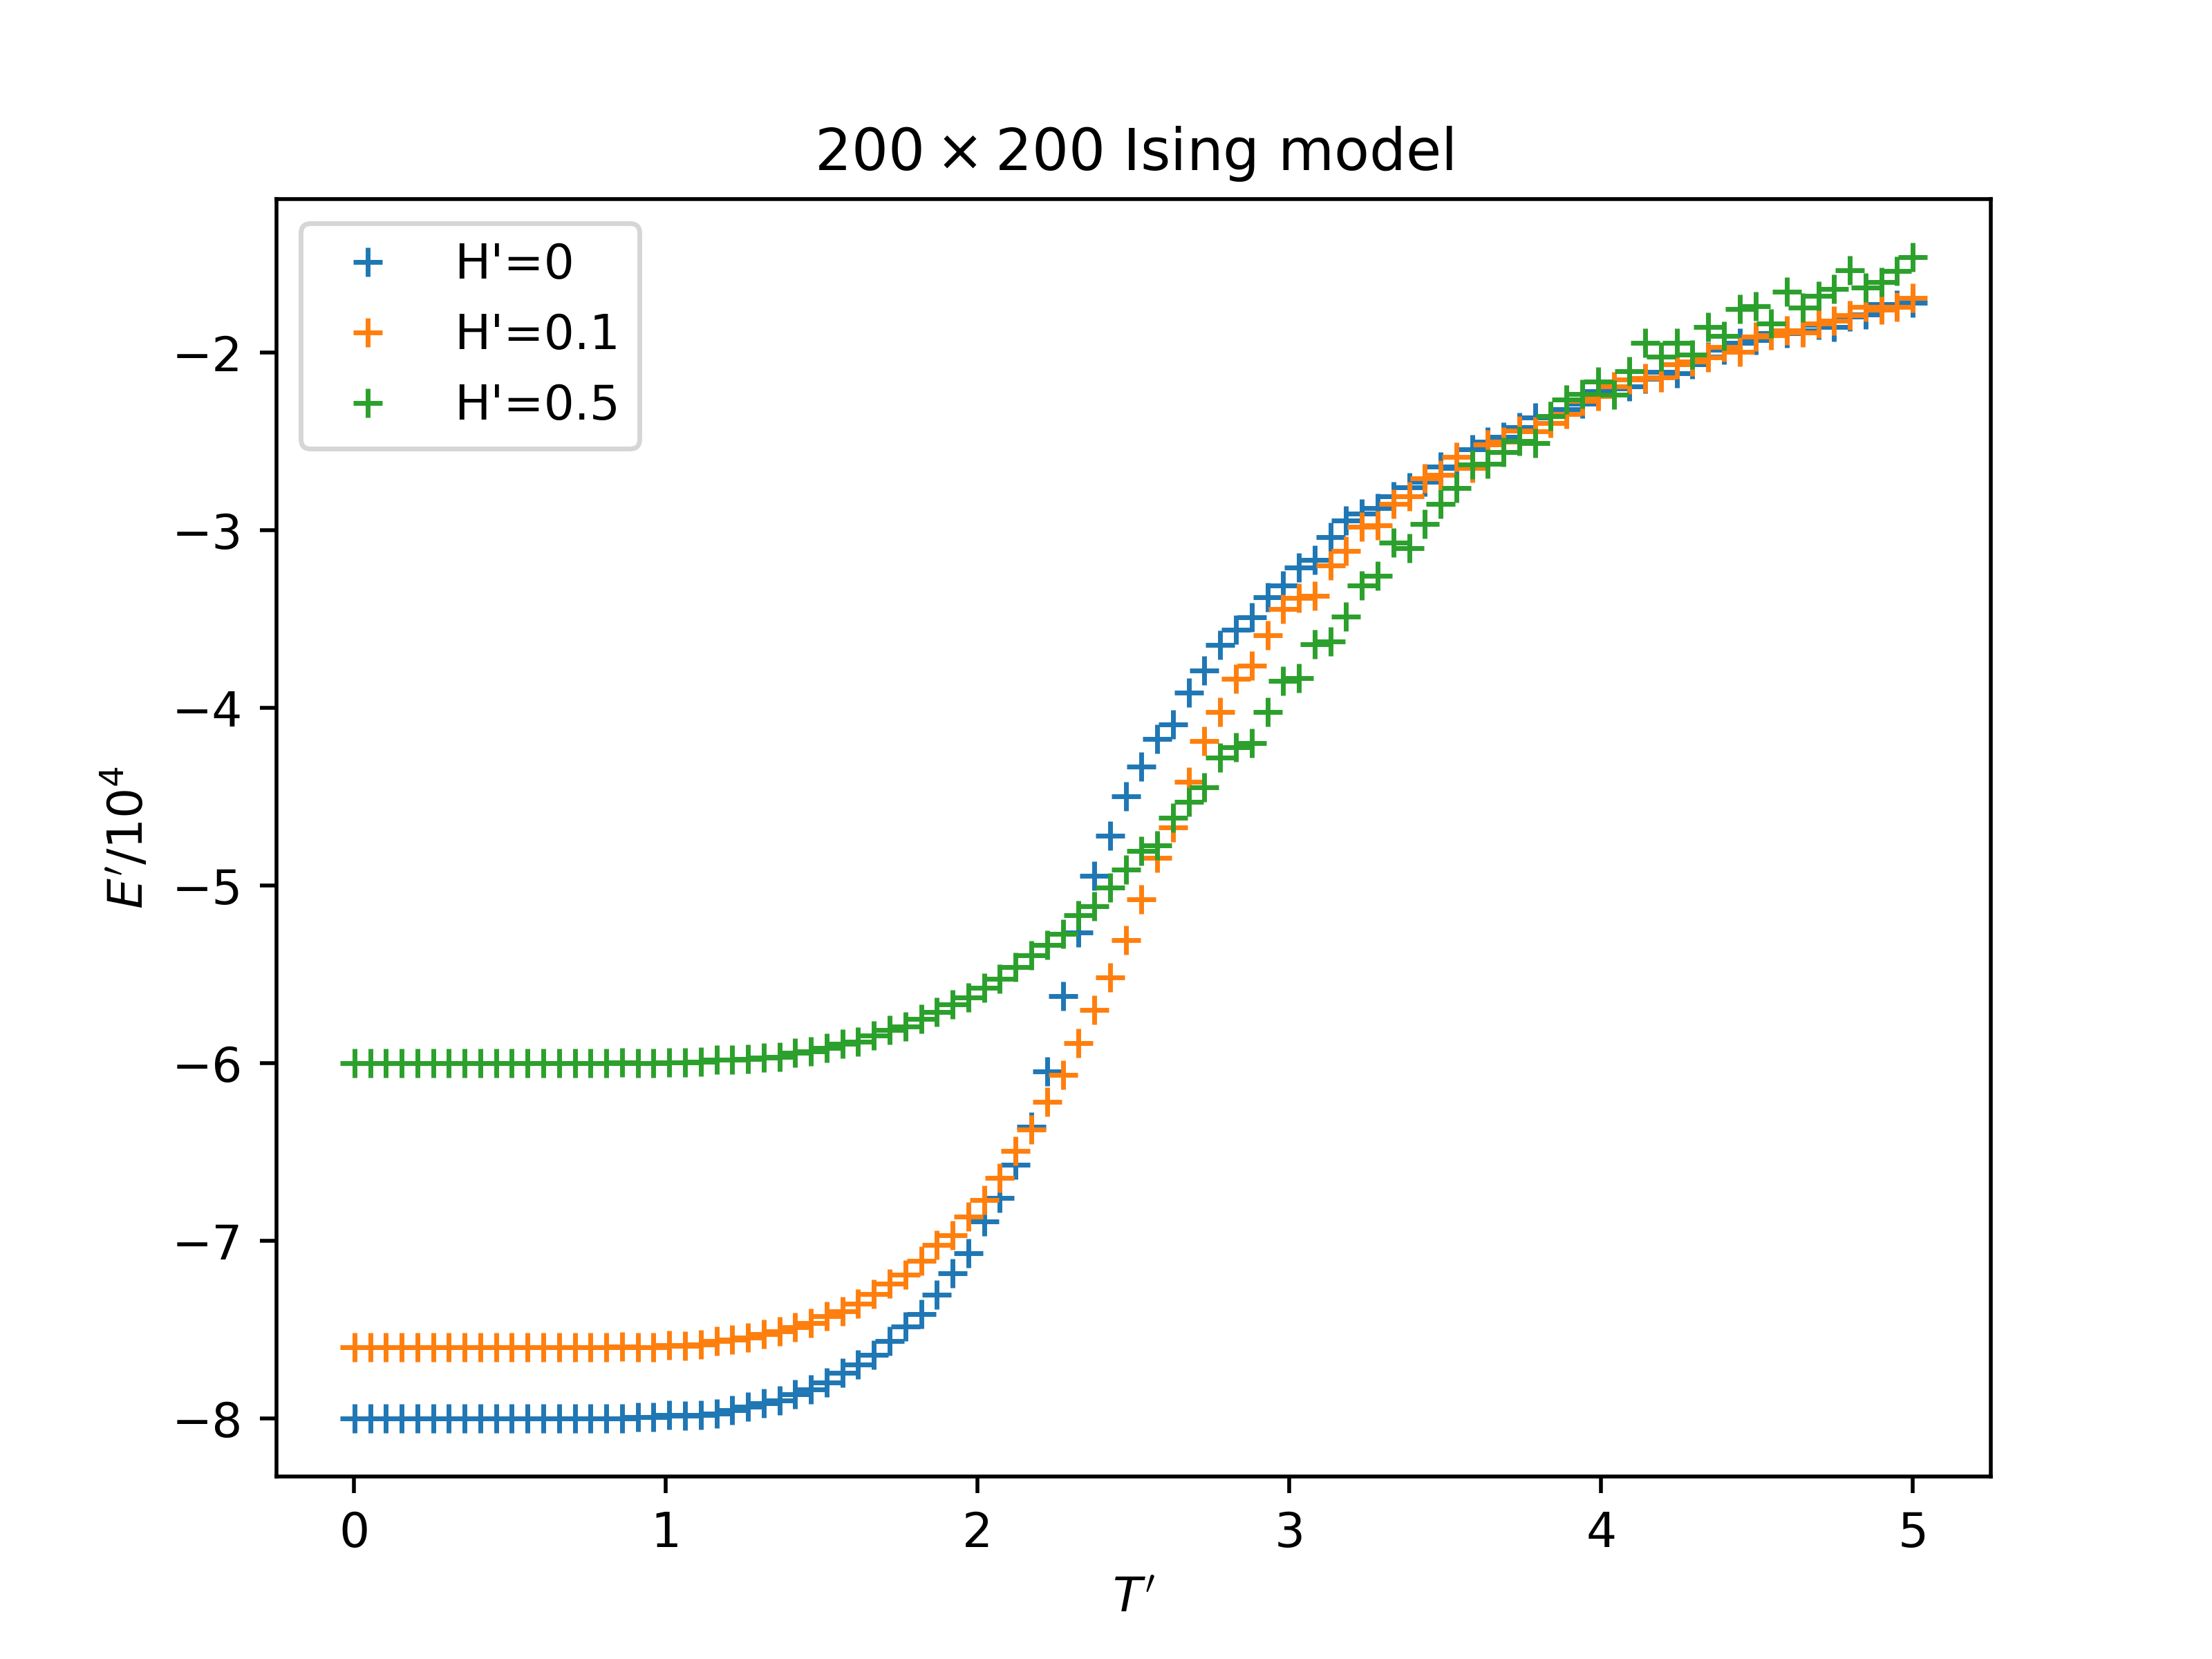
\includegraphics[width=0.48\textwidth]{plots/E-T_withB_diagram(latest,200).png}\hfill
    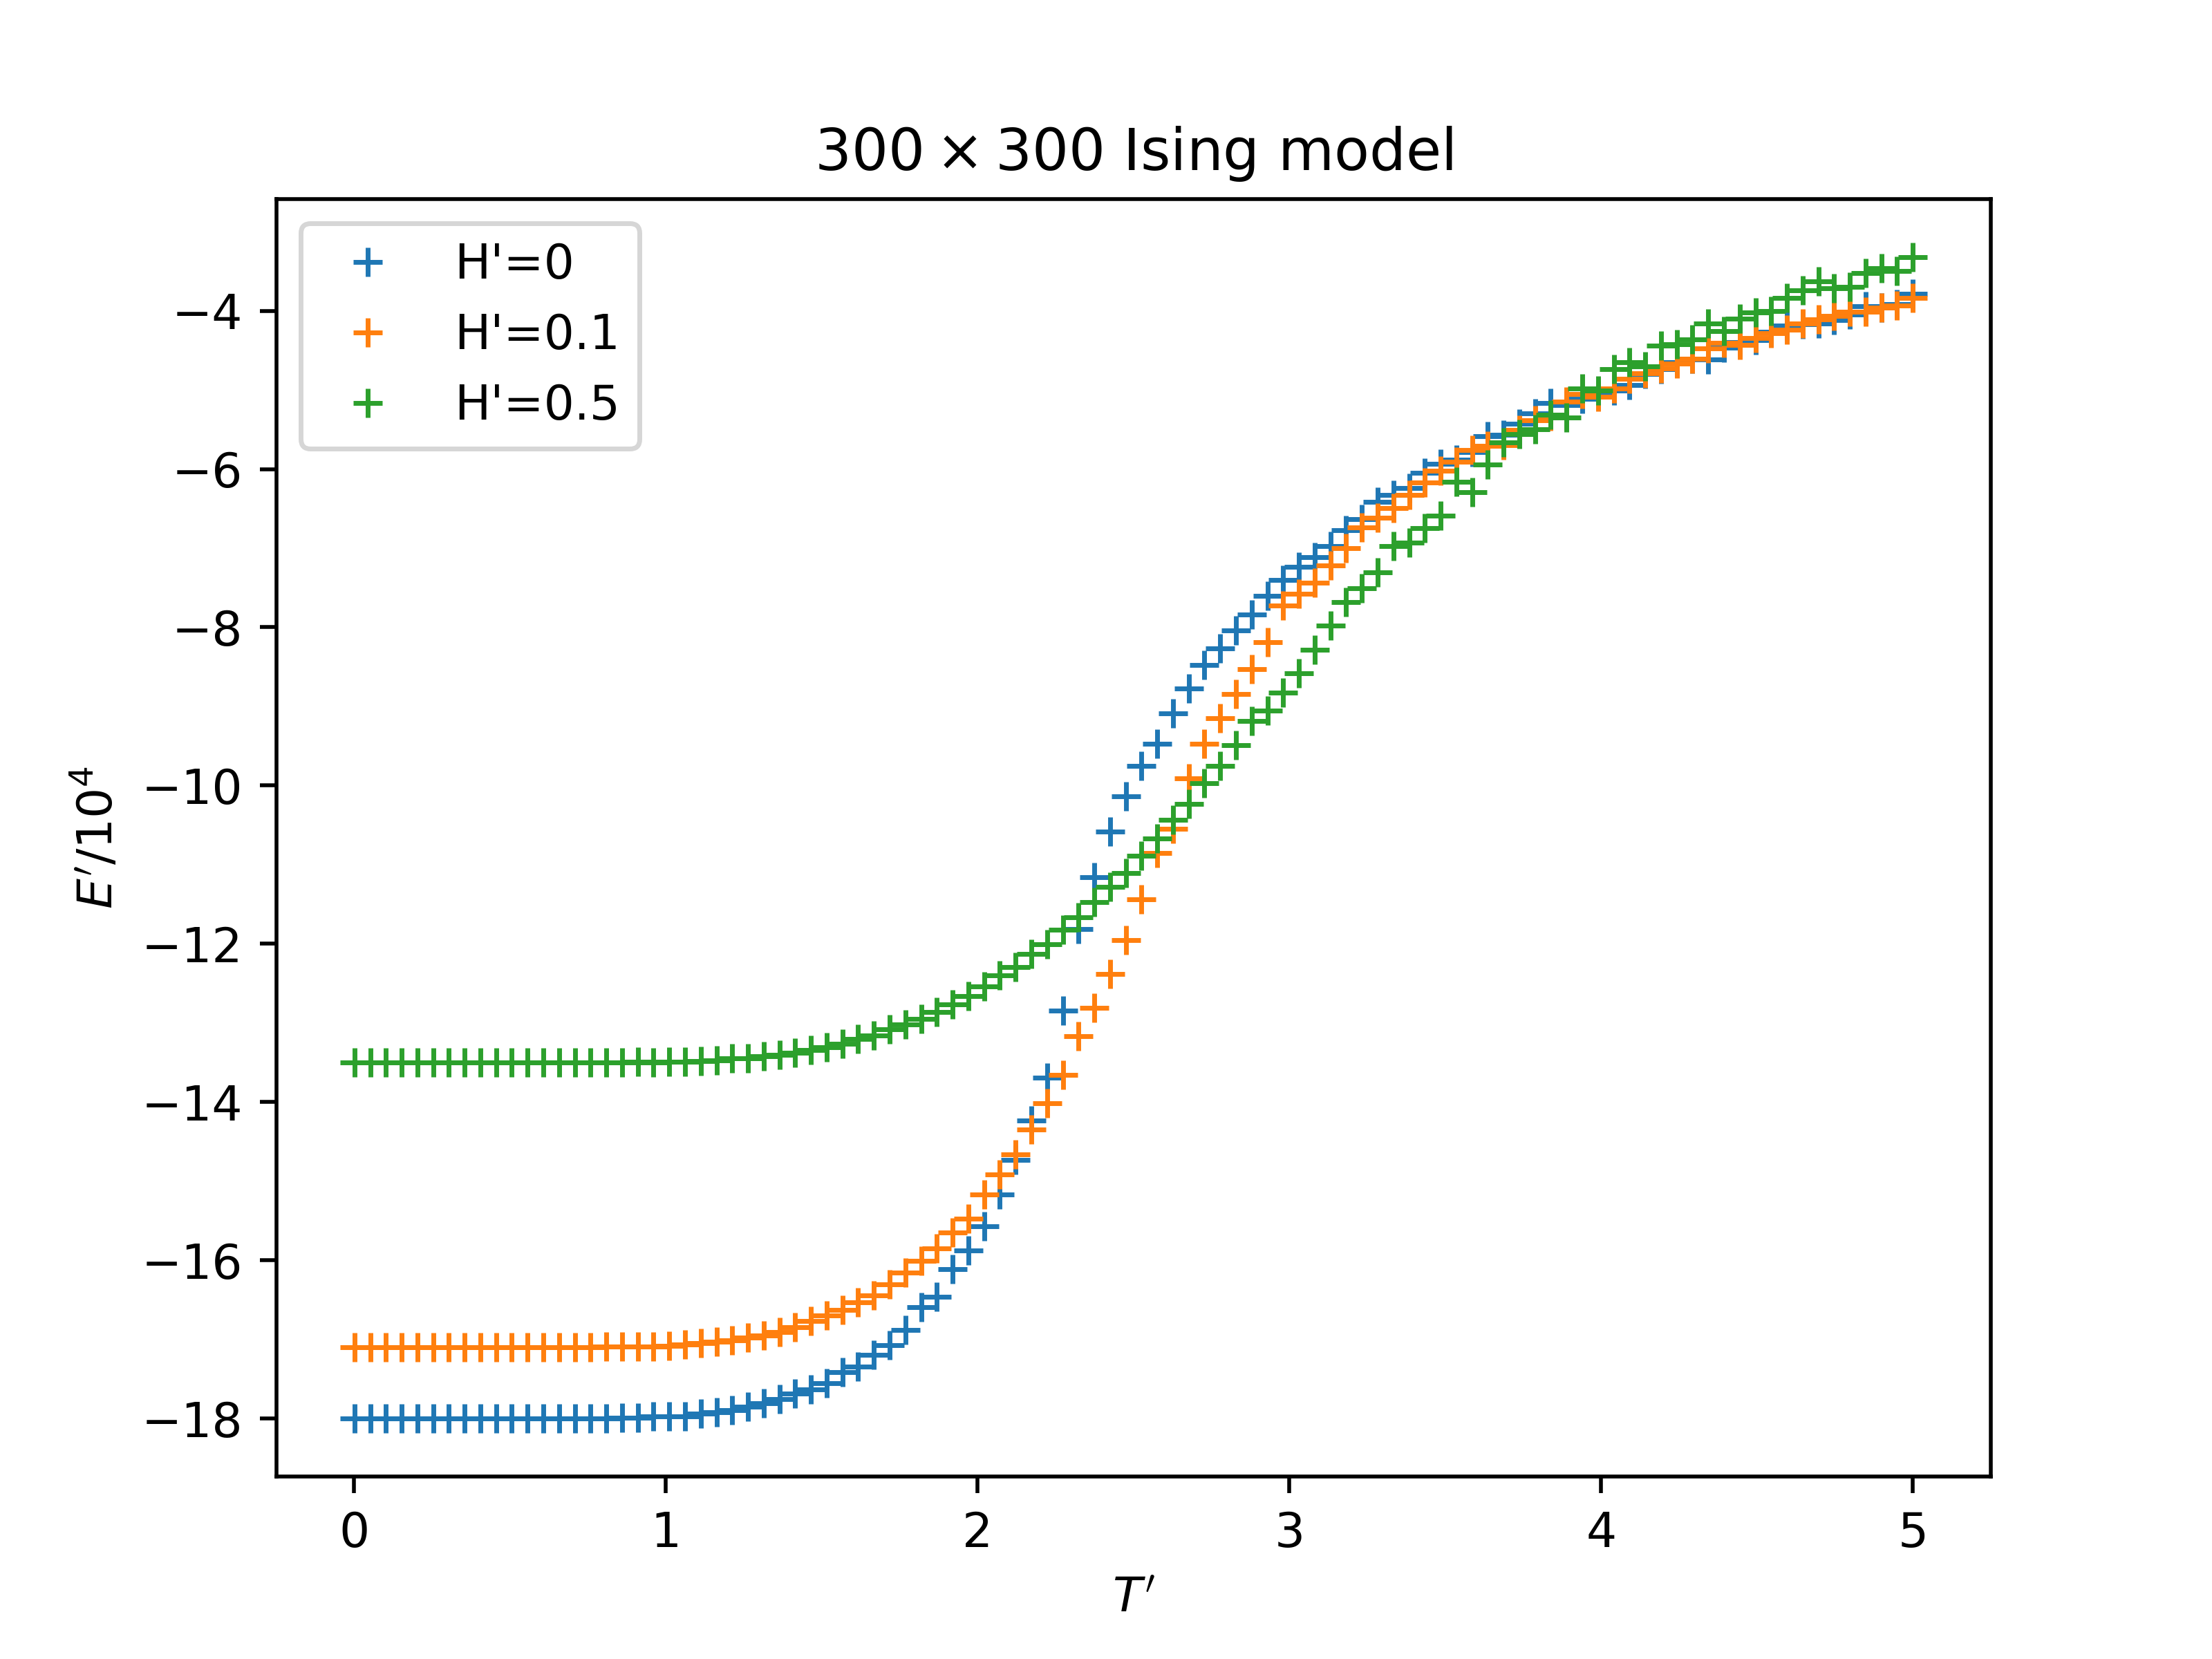
\includegraphics[width=0.48\textwidth]{plots/E-T_withB_diagram(latest,300).png}
    \caption{$E-T'$ relation of different system size $N$}
    \label{E-T/N}
\end{figure}

\begin{figure}
    \centering
    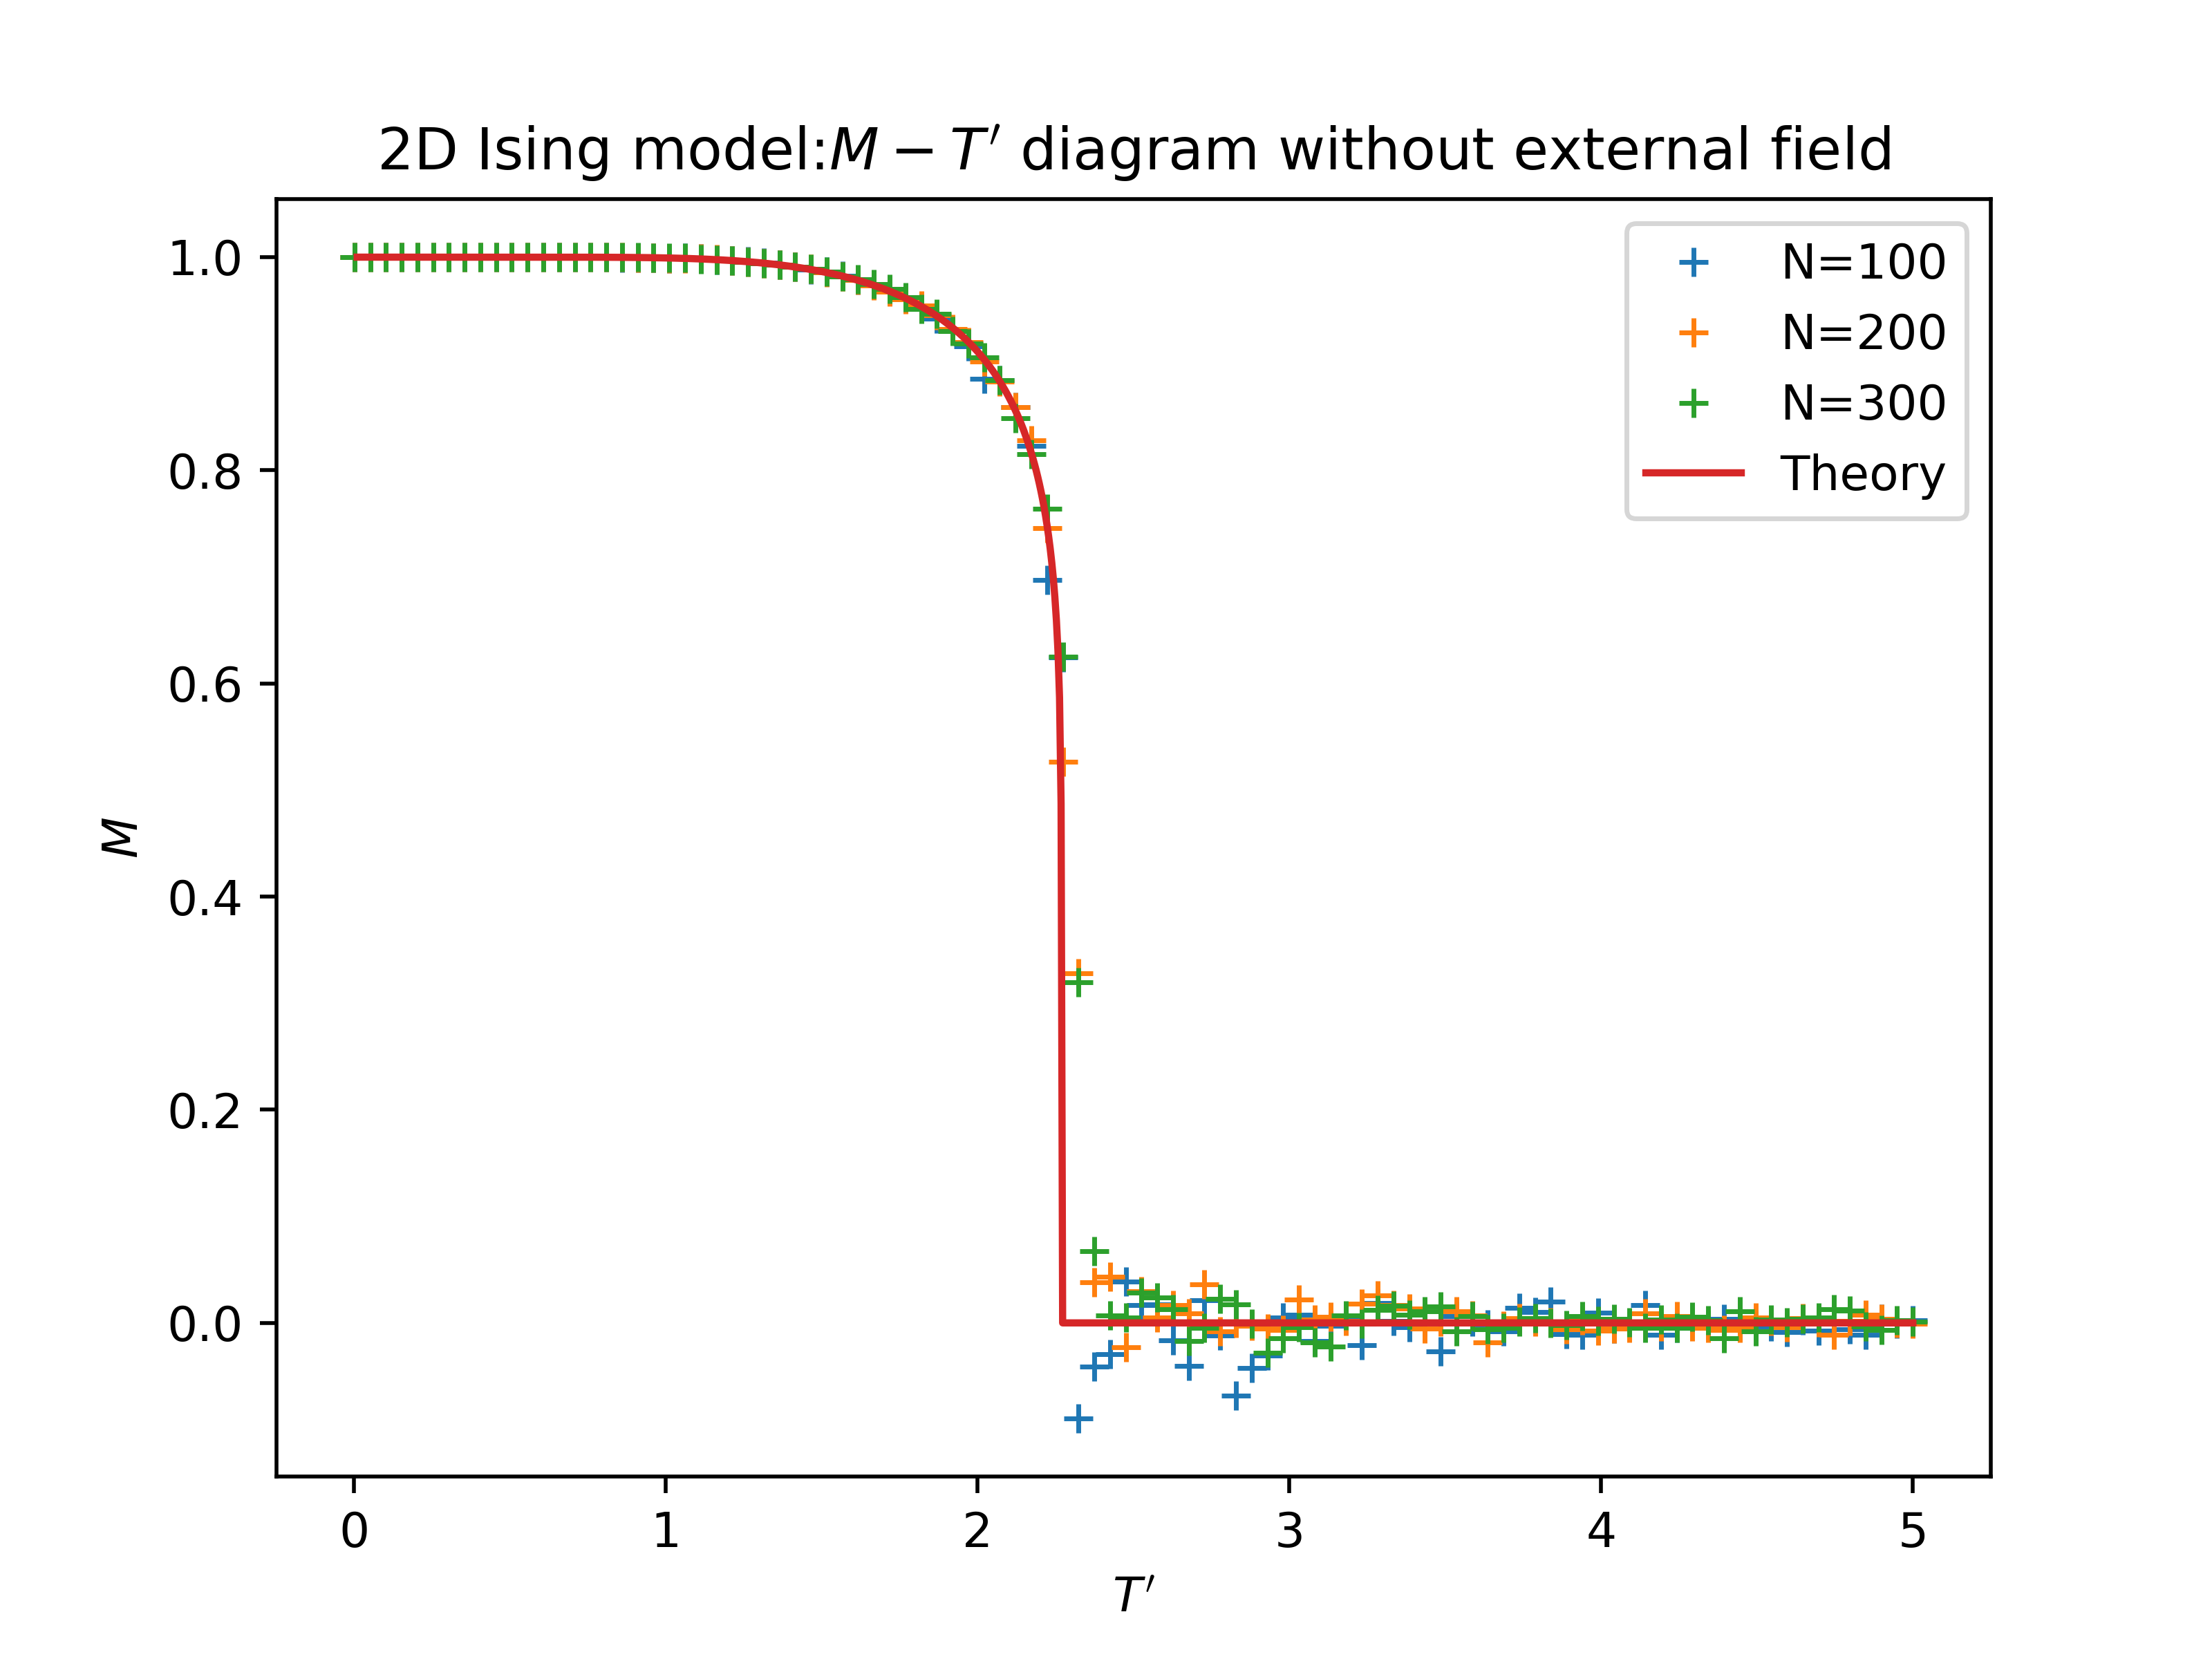
\includegraphics[width=0.8\linewidth]{plots/2D Ising model without external field.png}
    \caption{$E'-T'$ relation of different system size $N$}
    \label{noH}
\end{figure}

\subsubsection{Discussion on $\mathbb{Z}_2$ Symmetry}\label{Z2}

Theoretically, the Hamiltonian\ref{Hamiltonian} of our model satisfies a discrete $\mathbb{Z}_2$ symmetry. Such that the Hamiltonian remains unchanged under $s_i \rightarrow -s_i$(for all i) and $H \rightarrow -H$. From the formula of energy\ref{Hamiltonian} and magnetization\ref{magnetization}, we know that, under such $\mathbb{Z}_2$ transformation the hamiltonian remains invariant.

\begin{align}\label{z2case}
    &E \rightarrow E\\
    &M \rightarrow -M
\end{align}

We would like to test whether this symmetry is also preserved in numerical simulation. So we simulate the following two process(which is in $\mathbb{Z}_2$ symmetry to each other) and test whether this formula\ref{z2case} remains satisfied in the whole physical process:
\begin{itemize}
    \item Heating from zero temperature with positive $H$ and $s_i = 1 \quad(\forall i)$
    \item Heating from zero temperature with negative $H$ and $s_i = -1 \quad(\forall i)$
\end{itemize}

The approximate conservation of this $\mathbb{Z}_2$ symmetry can already be seen in previous diagram\ref{M-T/N}. The magnetization appears symmetric for positive and negative external field. In order to have a clearer metric on how good the $\mathbb{Z}_2$ symmetry is conserved during the heating process, we define a relative energy bias $\alpha_E$ and a relative magnetization bias $\alpha_M$:

\begin{align}
    &\alpha_E(H) = \frac{E(H)-E(-H)}{E(H)}\\
    &\alpha_M(H) = \frac{M(H)+M(-H)}{M(H)}
\end{align}

The $\mathbb{Z}_2$ symmetry is perfectly conserved if these two relative values are close to 0 and are completely broken if these values go to 1. We plot this $\alpha_E(H)$ and $\alpha_E(H)$ for a given $H$ and different temperature and system size here\ref{E-T/N}.

We can see from the diagram \ref{E-T/N} that $\alpha_E$ remains smaller than $0.05$ and $\alpha_M$ remains smaller than $0.15$ for all the temperatures. Moreover, we perform the statistical calculation \ref{tab:alphae} and \ref{tab:alpham} for $\alpha_E$ and $\alpha_M$ and see no systematic deviation from zero value. The expectation of $\alpha_E$ and $\alpha_M$ is much smaller than the standard variance. From this we draw our conclusion that we have not observe statistically clear evidence that the system breaks the $\mathbb{Z}_2$ symmetry when increasing the temperature.

The data also clearly indicates that for larger system the standard deviation of $\alpha_E$ and $\alpha_M$ is smaller. This is related to previous discussions on system size.\ref{smoothdiscussion}

% Table generated by Excel2LaTeX from sheet 'Sheet1'
\begin{table}[htbp]
  \centering
  \caption{Statistical analysis for $\alpha_E$}
    \begin{tabular}{|r|r|r|}
    \hline
    \multicolumn{1}{|l|}{N} & \multicolumn{1}{l|}{$\bar\alpha_E$} & \multicolumn{1}{l|}{$\sigma_{\alpha}$} \\
    \hline
    100  & 0.00053 & 0.0128 \\
    \hline
    200  & -0.00036 & 0.0088 \\
    \hline
    300  & -0.00068 & 0.0061 \\
    \hline
    \end{tabular}%
  \label{tab:alphae}%
\end{table}%

% Table generated by Excel2LaTeX from sheet 'Sheet1'
\begin{table}[htbp]
  \centering
  \caption{Statistical analysis for $\alpha_M$}
    \begin{tabular}{|r|r|r|}
    \hline
    \multicolumn{1}{|l|}{N} & \multicolumn{1}{l|}{$\bar\alpha_M$} & \multicolumn{1}{l|}{$\sigma_{\alpha}$} \\
    \hline
    100  & -0.0012 & 0.044 \\
    \hline
    200  & -0.0026 & 0.027 \\
    \hline
    300  & 0.0051 & 0.021 \\
    \hline
    \end{tabular}%
  \label{tab:alpham}%
\end{table}%


\begin{figure}\label{ETM}
    \centering
    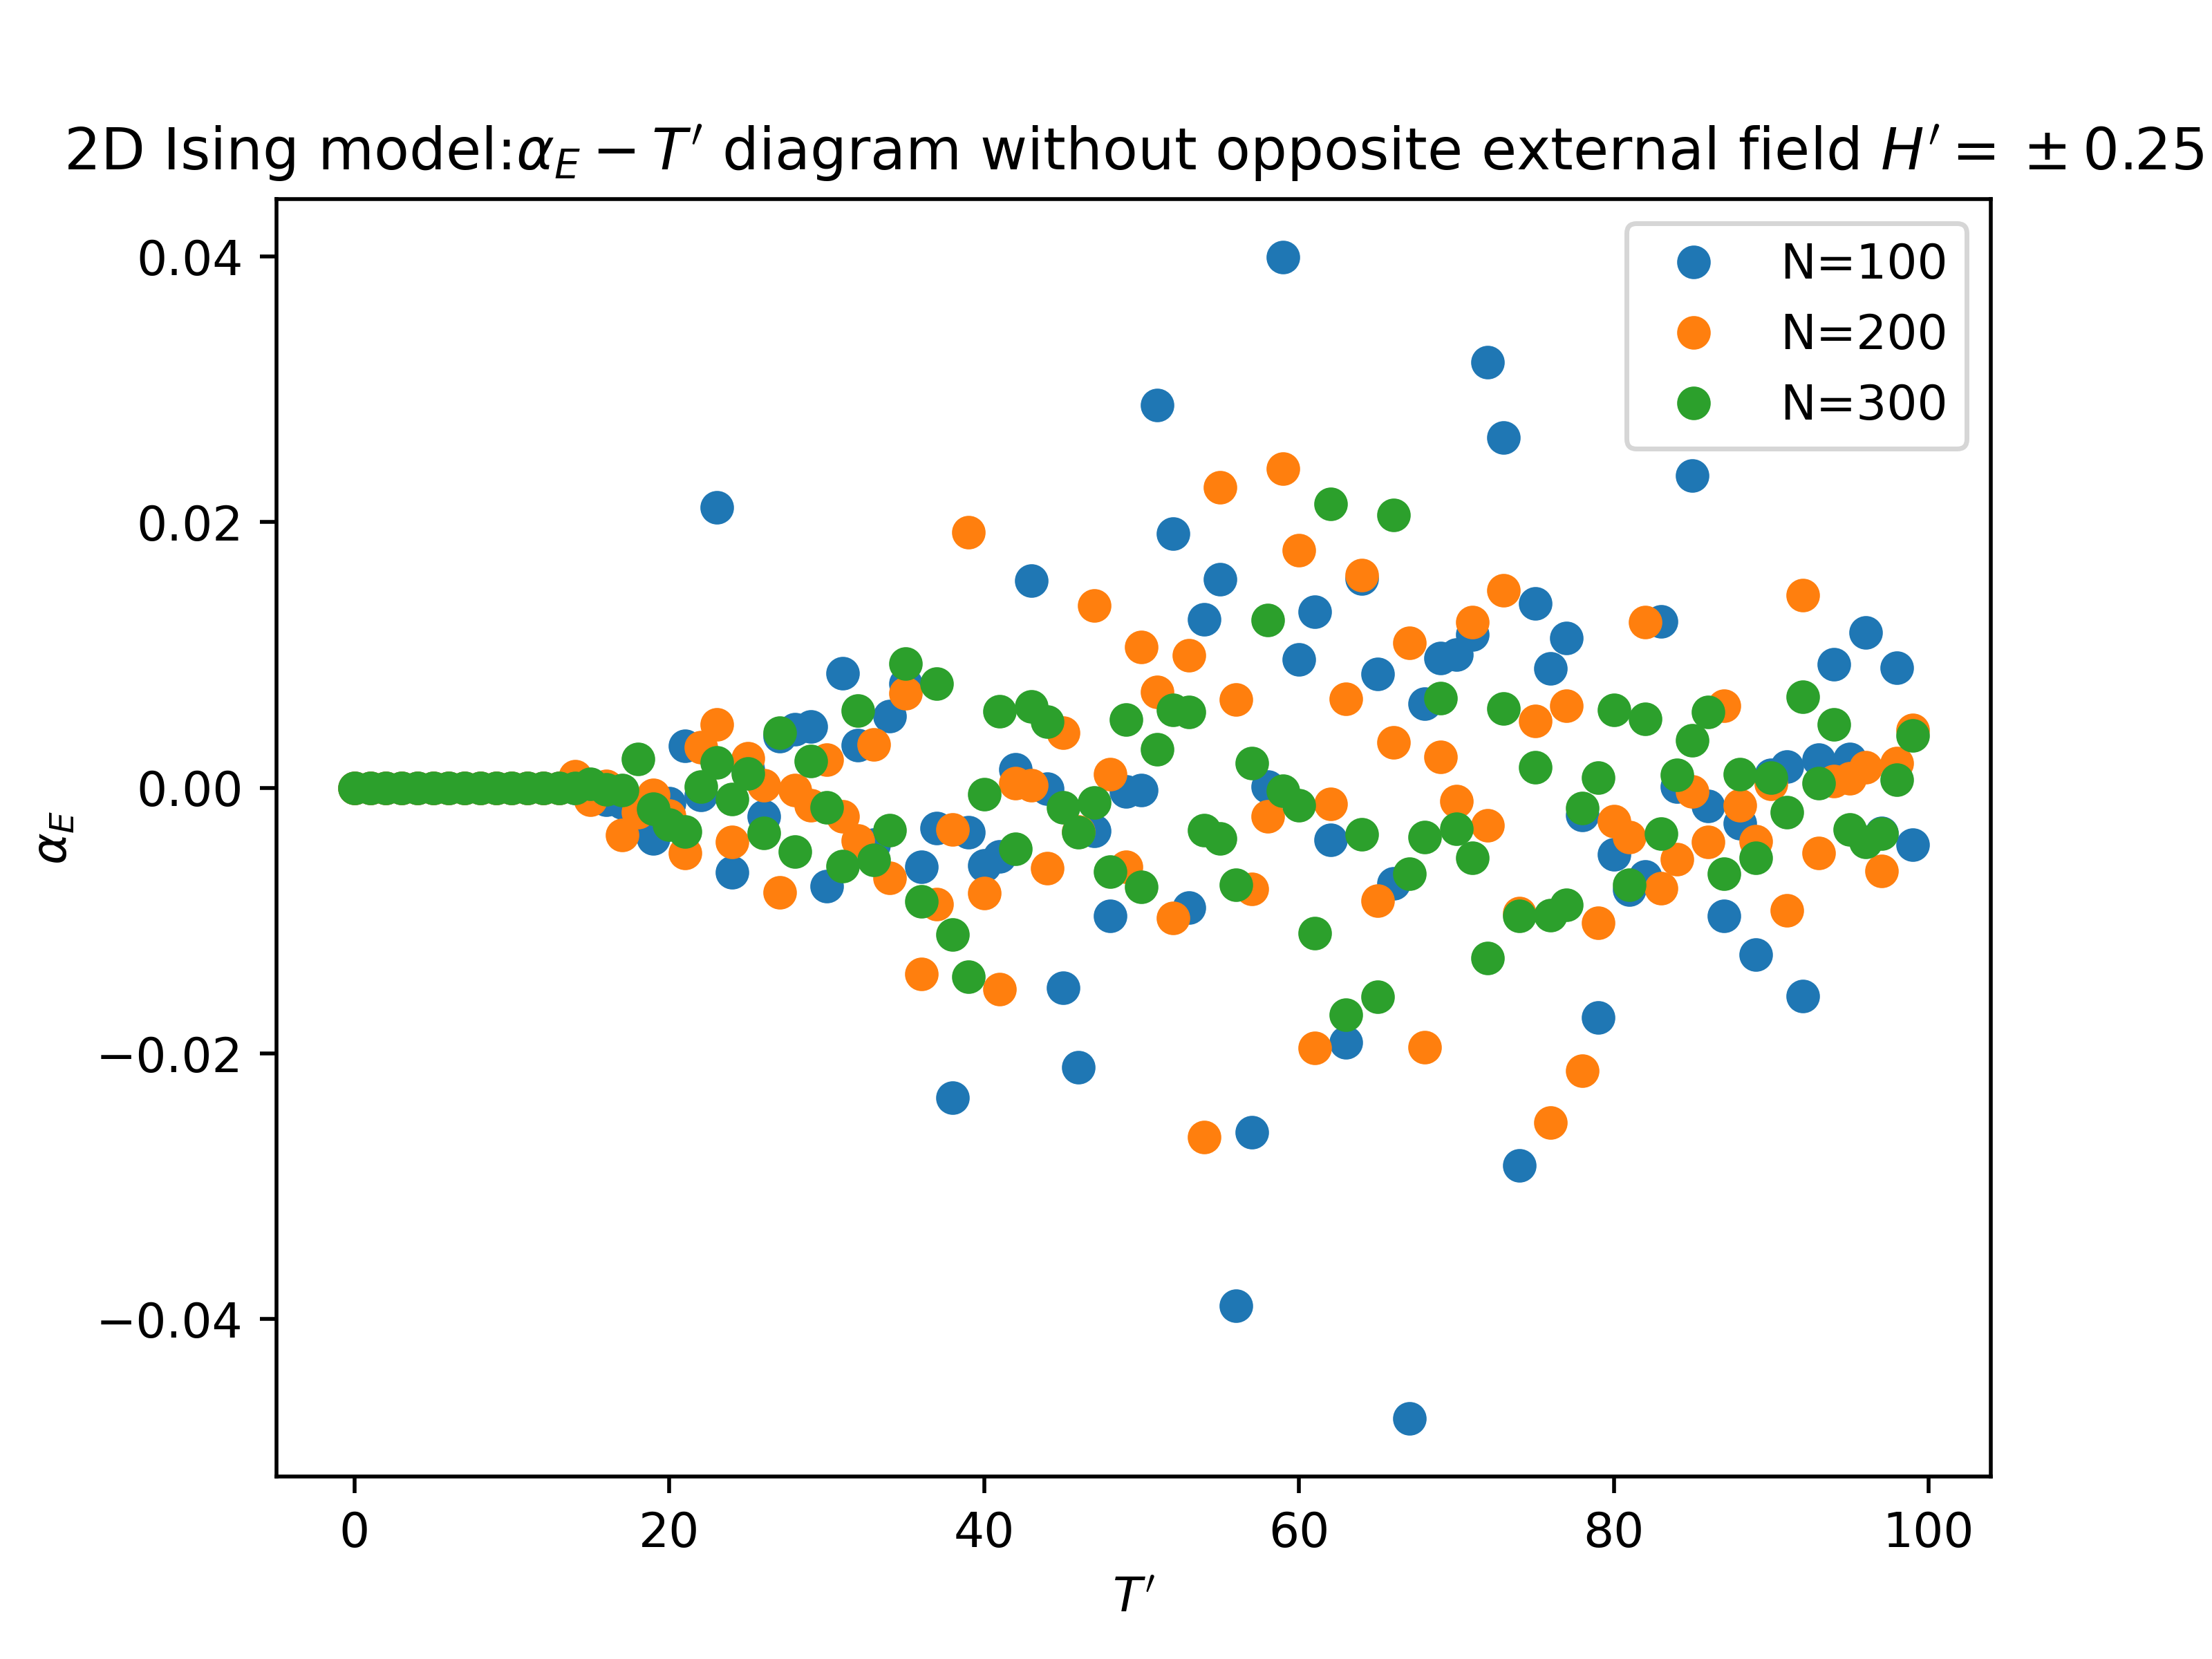
\includegraphics[width=0.48\textwidth]{plots/alphaE-T.png}\hfill
    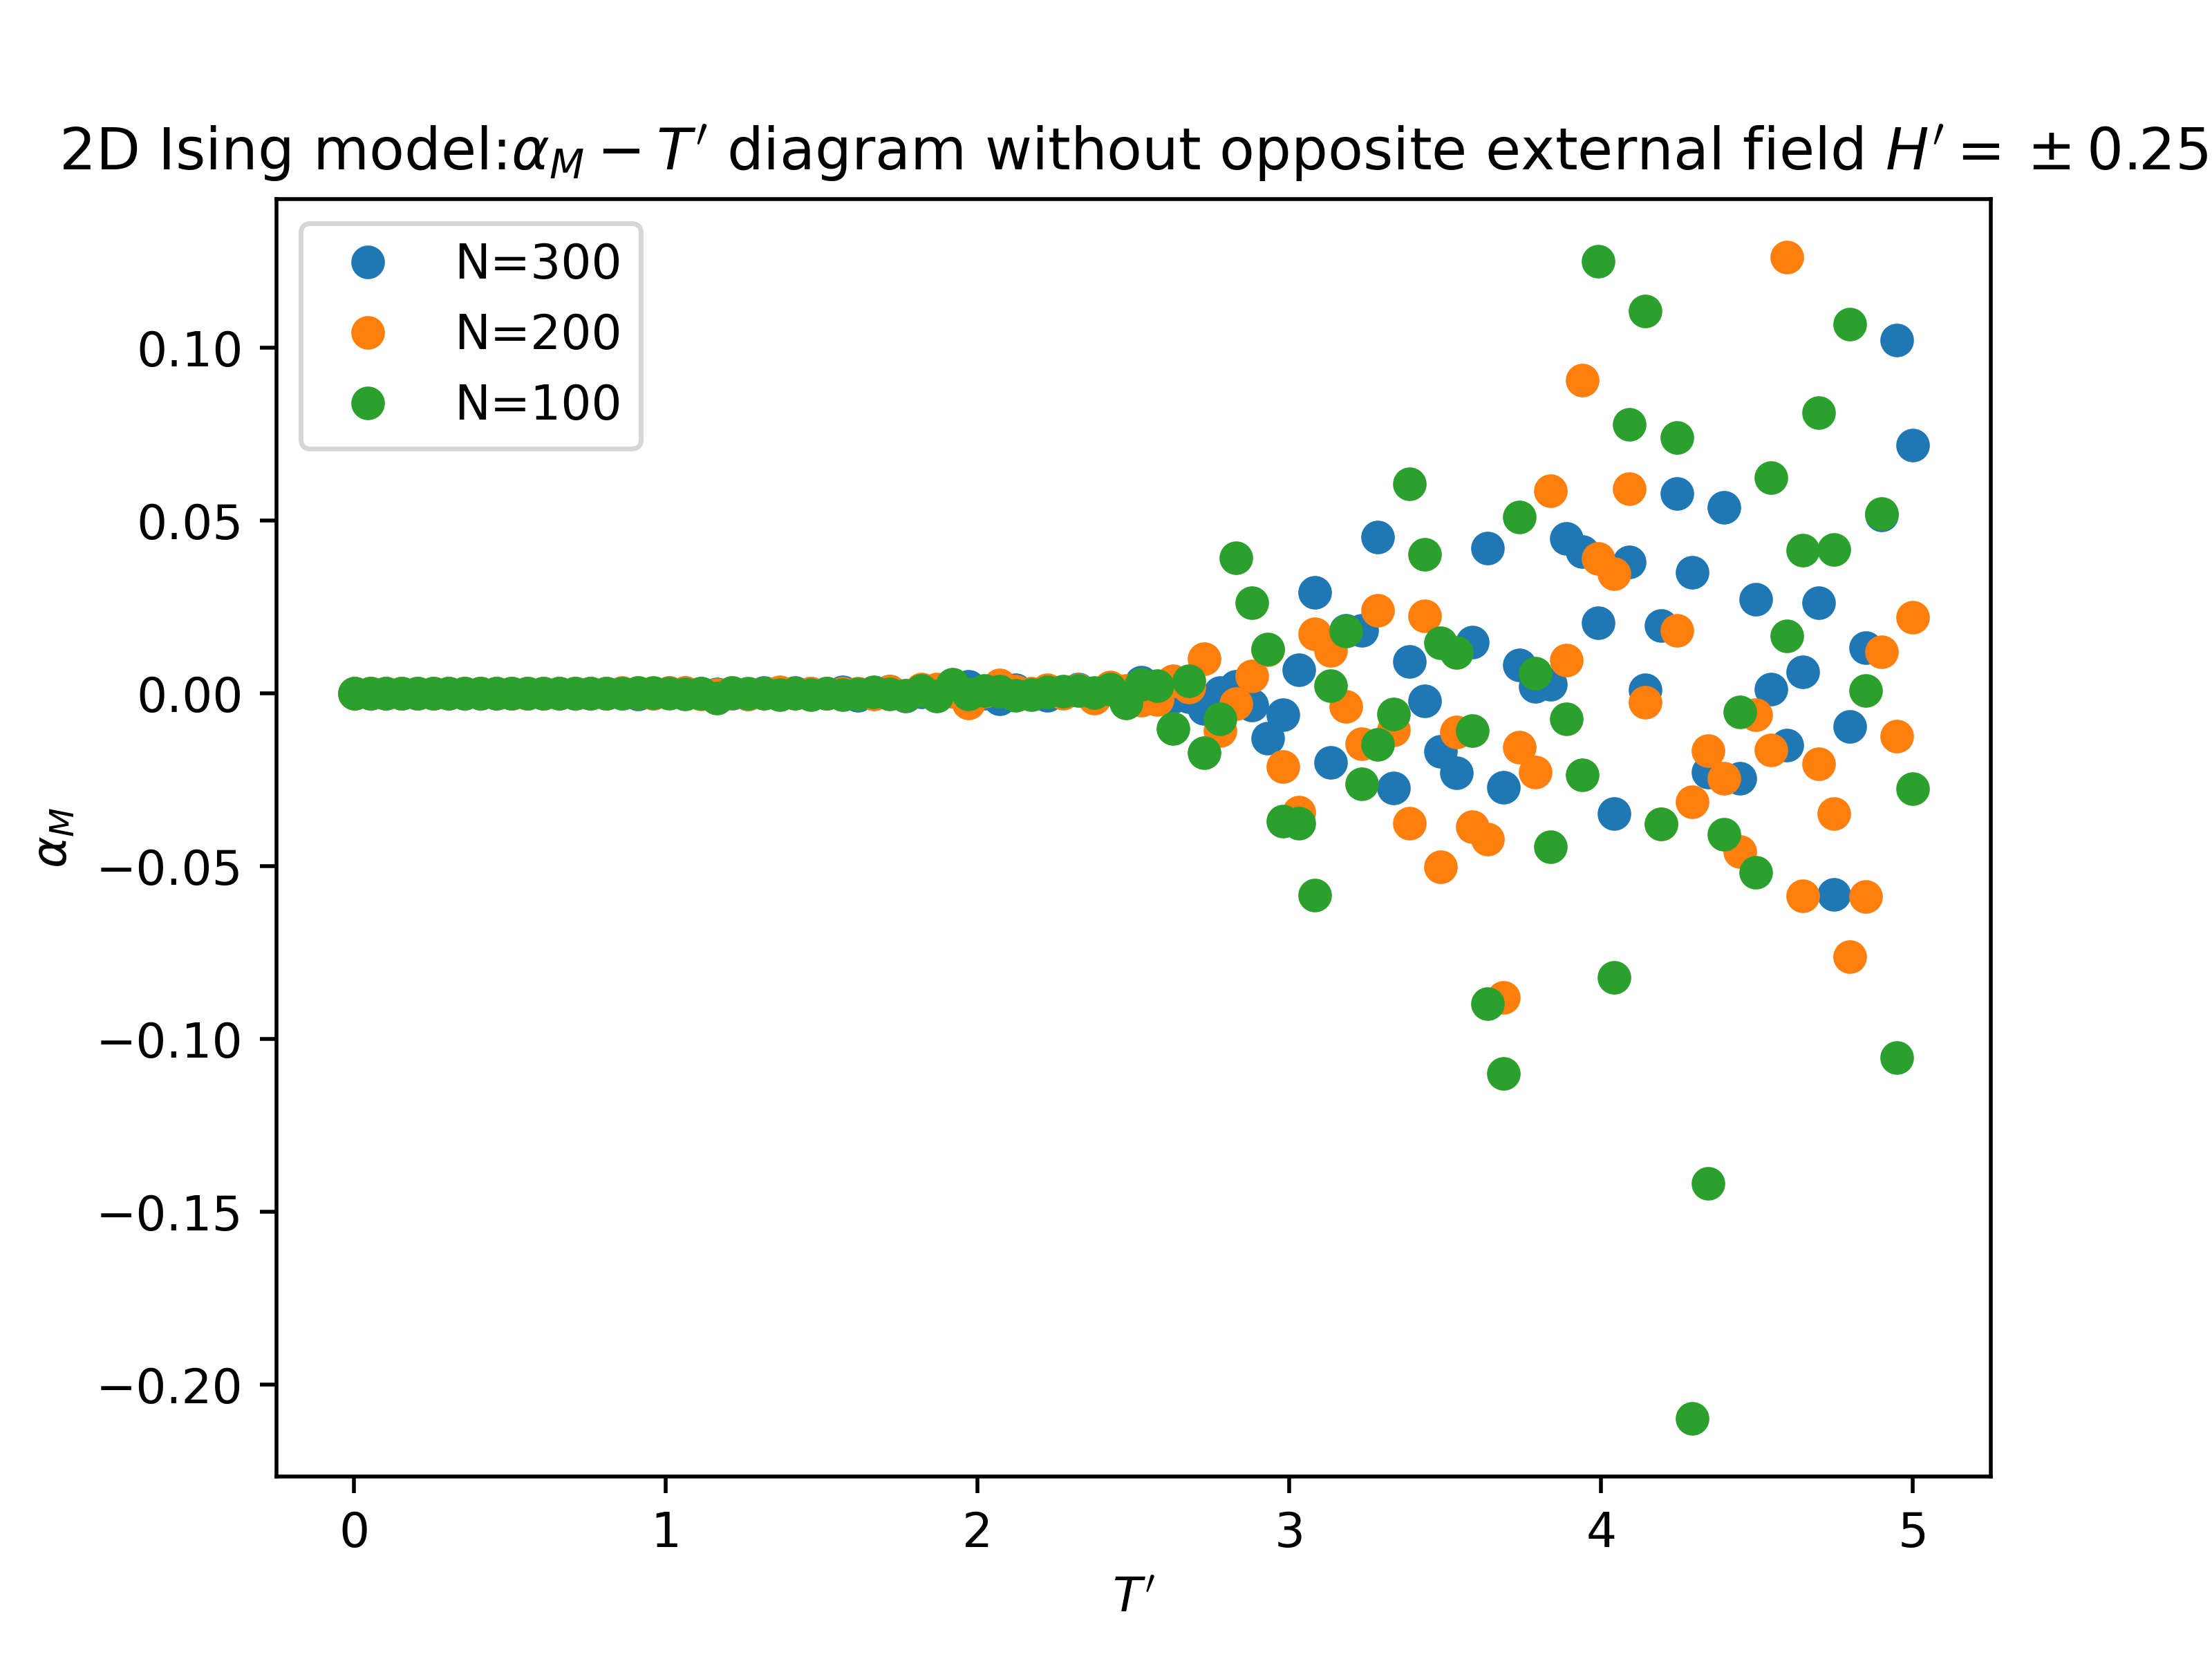
\includegraphics[width=0.48\textwidth]{plots/alphaM-T.png}
    \caption{The Testing of $\mathbb{Z}_2$ Symmetry Preservation}
    \label{E-T/N}
\end{figure}

\subsection{Heating from Metastable State}\label{heating1}
The source codes for this part can be found at: \url{https://github.com/rising1227/2DIsingModel.git}.

\subsubsection{Main Results}
Figures \ref{fig:meta50} and \ref{fig:meta500} show the $E^\prime$-$T^\prime$ and $M$-$T^\prime$ relations of a heating 2D Ising model initially with $M = 1$. If $H^\prime < 0$, the system is initially in a metastable state.

We find that the $E^\prime$-$T^\prime$ and $M$-$T^\prime$ curves for negative $H^\prime$ start to coincide with those for positive $H^\prime$ at certain temperatures. This indicates that the spins flipped to align with the magnetic field to minimize energy. The coincidence occurs at lower temperatures for larger magnitudes of $H^\prime$. This is because under our choices of $|H^\prime| < 8$, when the spins in the system are mainly pointing up, flipping a spin to point down increases the energy and is unfavorable. For larger magnitudes of $H^\prime$, the increase in energy is smaller and the flip is more likely to occur.

Furthermore, a comparison of Figures \ref{meta50El} and \ref{meta50Ml} with Figures \ref{meta500El} and \ref{meta500Ml} shows that the changes are sharper for smaller systems.

A comparison of Figures \ref{meta500Es} and \ref{meta500Ms} with Figures \ref{meta500El} and \ref{meta500Ml} shows that the changes are sharper when more Markov chain steps are taken.



\begin{figure}[H]
    \centering
    \begin{subfigure}[H]{0.48\textwidth}
        \centering
        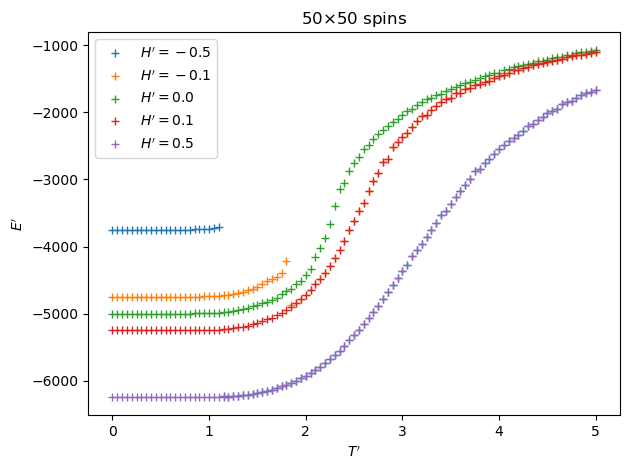
\includegraphics[width=\textwidth]{Meta/energy_N50_steps100000-10000000-2000000_Hsteps1000000.png}
        \caption{}
        \label{meta50Es}
    \end{subfigure}
    \hfill
    \centering
    \begin{subfigure}[H]{0.48\textwidth}
        \centering
        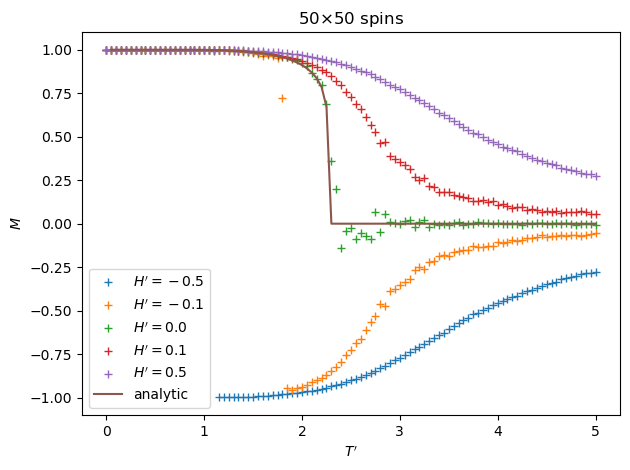
\includegraphics[width=\textwidth]{Meta/magnetization_N50_steps100000-10000000-2000000_Hsteps1000000.png}
        \caption{}
        \label{meta50Ms}
    \end{subfigure}

    \begin{subfigure}[H]{0.48\textwidth}
        \centering
        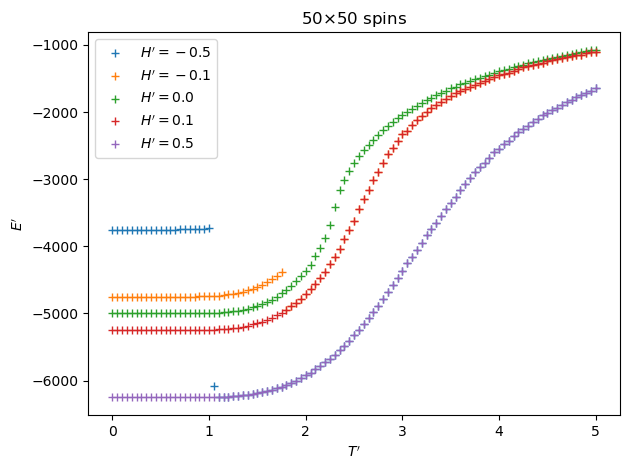
\includegraphics[width=\textwidth]{Meta/energy_N50_steps500000-50000000-10000000_Hsteps5000000.png}
        \caption{}
        \label{meta50El}
    \end{subfigure}
    \hfill
    \begin{subfigure}[H]{0.48\textwidth}
        \centering
        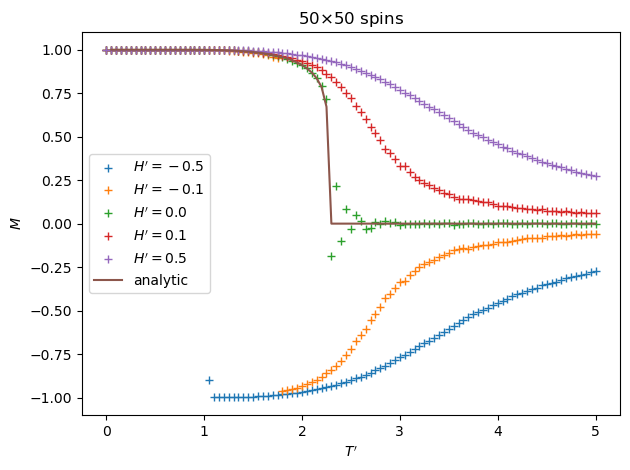
\includegraphics[width=\textwidth]{Meta/magnetization_N50_steps500000-50000000-10000000_Hsteps5000000.png}
        \caption{}
        \label{meta50Ml}
    \end{subfigure}
    \caption{$E^\prime$-$T^\prime$ and $M$-$T^\prime$ relations for a $N = 50$ heating 2D Ising model initially with $M = 1$. If $H^\prime < 0$, the system is initially in a metastable state. In (a) and (b), for the $H^\prime = 0$ curve, $1 \times 10^5$, $1 \times 10^7$, and $2 \times 10^6$ Markov chain steps are taken respectively for $0 < T^\prime < 2.1$, $2.1 \leq T^\prime \leq 2.5$, and $2.5 < T^\prime < 5$. For the $H^\prime \neq 0$ curves, $1 \times 10^6$ steps are taken. In (c) and (d), the steps are five times larger. That is, for the $H^\prime = 0$ curve, $5 \times 10^5$, $5 \times 10^7$, and $1 \times 10^7$ Markov chain steps are taken respectively. For the $H^\prime \neq 0$ curves, $5 \times 10^6$ steps are taken.}
    \label{fig:meta50}
\end{figure}

\begin{figure}[H]
    \centering
    \begin{subfigure}[H]{0.48\textwidth}
        \centering
        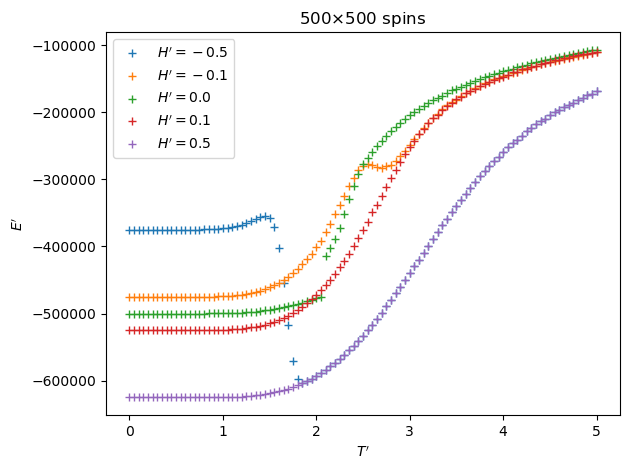
\includegraphics[width=\textwidth]{Meta/energy_N500_steps300000-30000000-6000000_Hsteps3000000.png}
        \caption{}
        \label{meta500Es}
    \end{subfigure}
    \hfill
    \centering
    \begin{subfigure}[H]{0.48\textwidth}
        \centering
        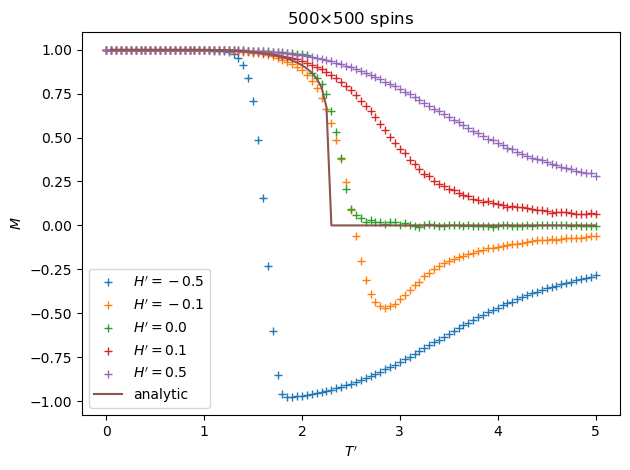
\includegraphics[width=\textwidth]{Meta/magnetization_N500_steps300000-30000000-6000000_Hsteps3000000.png}
        \caption{}
        \label{meta500Ms}
    \end{subfigure}

    \begin{subfigure}[H]{0.48\textwidth}
        \centering
        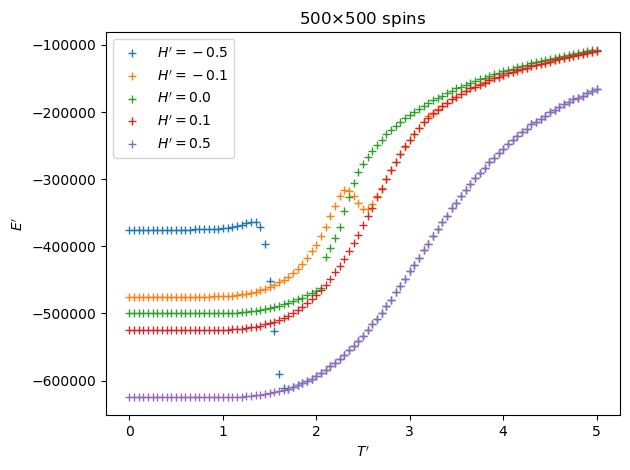
\includegraphics[width=\textwidth]{Meta/energy_N500_steps500000-50000000-10000000_Hsteps5000000.png}
        \caption{}
        \label{meta500El}
    \end{subfigure}
    \hfill
    \begin{subfigure}[H]{0.48\textwidth}
        \centering
        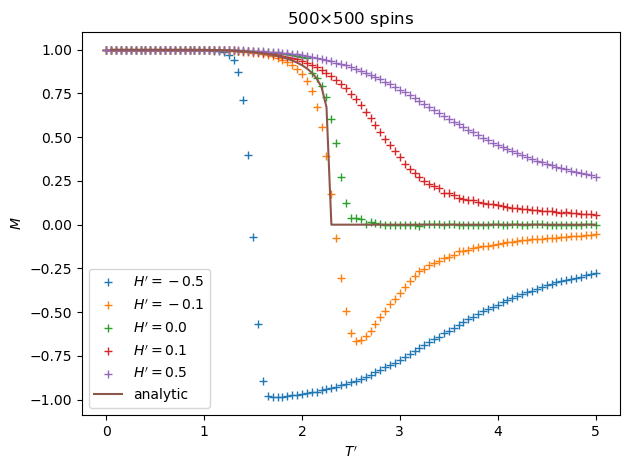
\includegraphics[width=\textwidth]{Meta/magnetization_N500_steps500000-50000000-10000000_Hsteps5000000.png}
        \caption{}
        \label{meta500Ml}
    \end{subfigure}
    \caption{$E^\prime$-$T^\prime$ and $M$-$T^\prime$ relations for a $N = 500$ heating 2D Ising model initially with $M = 1$. If $H^\prime < 0$, the system is initially in a metastable state. In (a) and (b), for the $H^\prime = 0$ curve, $3 \times 10^5$, $3 \times 10^7$, and $6 \times 10^6$ Markov chain steps are taken respectively for $0 < T^\prime < 2.1$, $2.1 \leq T^\prime \leq 2.5$, and $2.5 < T^\prime < 5$. For the $H^\prime \neq 0$ curves, $3 \times 10^6$ steps are taken. In (c) and (d), the steps are 5/3 times larger. That is, for the $H^\prime = 0$ curve, $5 \times 10^5$, $5 \times 10^7$, and $1 \times 10^7$ Markov chain steps are taken respectively. For the $H^\prime \neq 0$ curves, $5 \times 10^6$ steps are taken.}
    \label{fig:meta500}
\end{figure}

\subsubsection{Discussion on Convergence Problem}

Convergence problem is always something we need to take special care about in our metropolis algorithm. However, for the scenario of heating from true ground state, we can always ensure that an thermal equilibrium is achieved by continuously increasing the number of iteration. This is not true for the case of heating from metastable state. In the previous result, we have observed that for low temperature the system cannot move from metastable state to true ground state in large metropolis steps. 

We explained this phenomena by suggesting that the anti-aligned state is too stable for low temperature and thus requires very large iteration steps(larger than what a computer simulation can do) to move to its real ground state. This statement is physical since if the temperature is low and a real magnet is in the anti-aligned magnetization, this magnet is physically stable. We prove our explanation by increasing and decreasing the number of metropolis steps.

\subsection{Cooling from High Temperature}\label{cooling}

Figure \ref{fig:cool50} shows the $E^\prime$-$T^\prime$ and $M$-$T^\prime$ relations for a $N = 500$ 2D Ising model. The system is initially at $T^\prime = 5$ with random spin orientations and is then cooled down.

We find that the $M$-$T^\prime$ curve for $H^\prime = 0$ agrees with the analytical behavior in Figures \ref{coolMl} and \ref{coolMs}. The $M$-$T^\prime$ curve for $H^\prime = 0$ may randomly end up at $M = \pm 1$ because we are now starting with a random spin configuration and cooling down.

The $E^\prime$-$T^\prime$ curves for negative $H^\prime$ coincide with those for positive $H^\prime$ everywhere. The $M$-$T^\prime$ curves for negative $H^\prime$ are symmetric to those for positive $H^\prime$ everywhere. These results reflect the symmetry of the system.

\begin{figure}[H]
    \centering
    \begin{subfigure}[H]{0.48\textwidth}
        \centering
        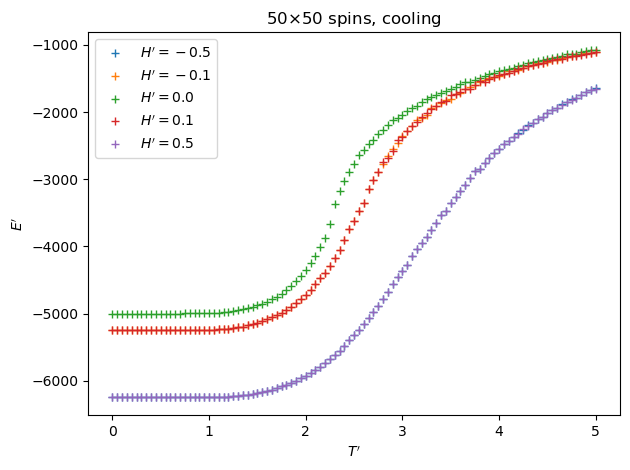
\includegraphics[width=\textwidth]{Cool/cool_energy_N50_steps2000000-10000000_Hsteps1000000.png}
        \caption{}
        \label{coolEs}
    \end{subfigure}
    \hfill
    \centering
    \begin{subfigure}[H]{0.48\textwidth}
        \centering
        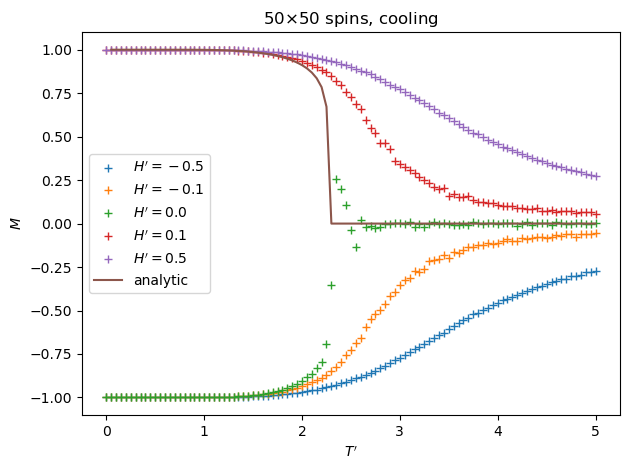
\includegraphics[width=\textwidth]{Cool/cool_magnetization_N50_steps2000000-10000000_Hsteps1000000.png}
        \caption{}
        \label{coolMs}
    \end{subfigure}

    \begin{subfigure}[H]{0.48\textwidth}
        \centering
        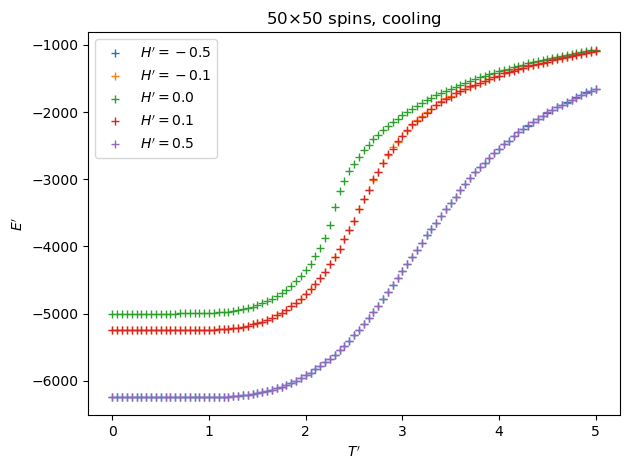
\includegraphics[width=\textwidth]{Cool/cool_energy_N50_steps10000000-50000000_Hsteps5000000.png}
        \caption{}
        \label{coolEl}
    \end{subfigure}
    \hfill
    \begin{subfigure}[H]{0.48\textwidth}
        \centering
        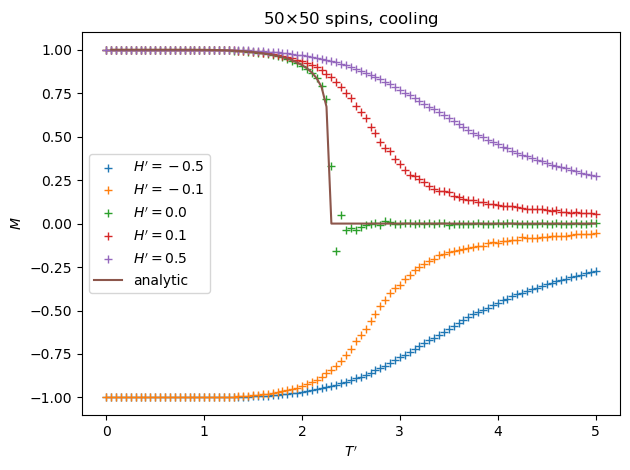
\includegraphics[width=\textwidth]{Cool/cool_magnetization_N50_steps10000000-50000000_Hsteps5000000.png}
        \caption{}
        \label{coolMl}
    \end{subfigure}
    \caption{$E^\prime$-$T^\prime$ and $M$-$T^\prime$ relations for a $N = 500$ 2D Ising model. The system is initially at $T^\prime = 5$ with random spin orientations and is then cooled down. In (a) and (b), for the $H^\prime = 0$ curve, $1 \times 10^7$ Markov chain steps are taken for $2.1 \leq T^\prime \leq 2.5$, and $2 \times 10^6$ steps are taken otherwise. For the $H^\prime \neq 0$ curves, $1 \times 10^6$ steps are taken. In (c) and (d), the steps are five times larger. That is, for the $H^\prime = 0$ curve, $5 \times 10^7$ Markov chain steps are taken for $2.1 \leq T^\prime \leq 2.5$, and $1 \times 10^7$ steps are taken otherwise. For the $H^\prime \neq 0$ curves, $5 \times 10^6$ steps are taken.}
    \label{fig:cool50}
\end{figure}


\section{Bonus: Results on Non-Static External Magnetic Field}\label{result2}

The source code for the bonus results can be found at the following link: 
\href{https://github.com/Salarscwise/simulation/tree/main/spin%20model%20variating%20H}{bonus source code}.




\subsection{Implementation Strategy}

The 2D Ising model with an oscillating external magnetic field was implemented using the Metropolis Monte Carlo algorithm on a 50 * 50 spin lattice. The key modifications to incorporate the time-dependent field were:

\begin{equation}
H(t) = H_0 \sin(\omega t)
\end{equation}

where $H_0$ is the field amplitude and $\omega$ is the angular frequency. The field was updated at each Monte Carlo step, affecting the energy difference calculation in the Metropolis algorithm:

\begin{equation}
\Delta E = 2J s_i \sum_{nn} s_j + 2H(t)s_i
\end{equation}

where $s_i$ is the spin being flipped, and the sum runs over nearest neighbors. The acceptance probability remains:

\begin{equation}
P(\Delta E) = \min(1, e^{-\beta \Delta E})
\end{equation}

\subsection{Energy Behavior}


Figure~\ref{fig:energy} illustrates the total lattice energy as a function of temperature for different field frequencies. Several key features emerge from this analysis. 

At zero temperature ($T=0$), the system under a static field reaches its lowest energy state, $E = -2N^2J - NH_0$. In contrast, oscillating fields result in higher energies due to the time-averaged field contribution being zero. 

In the critical region, around $T \approx 2.27$, a distinct phase transition is observed. This transition is characterized by a sharp change in energy, which becomes most pronounced near the critical temperature $T_c$. 

Frequency dependence further highlights the dynamical nature of the system. Higher frequencies consistently lead to elevated energy levels, reflecting the system's inability to fully respond to rapid oscillations of the external field. This incomplete relaxation underscores the impact of dynamical effects on the system's behavior.

\begin{figure}[h]
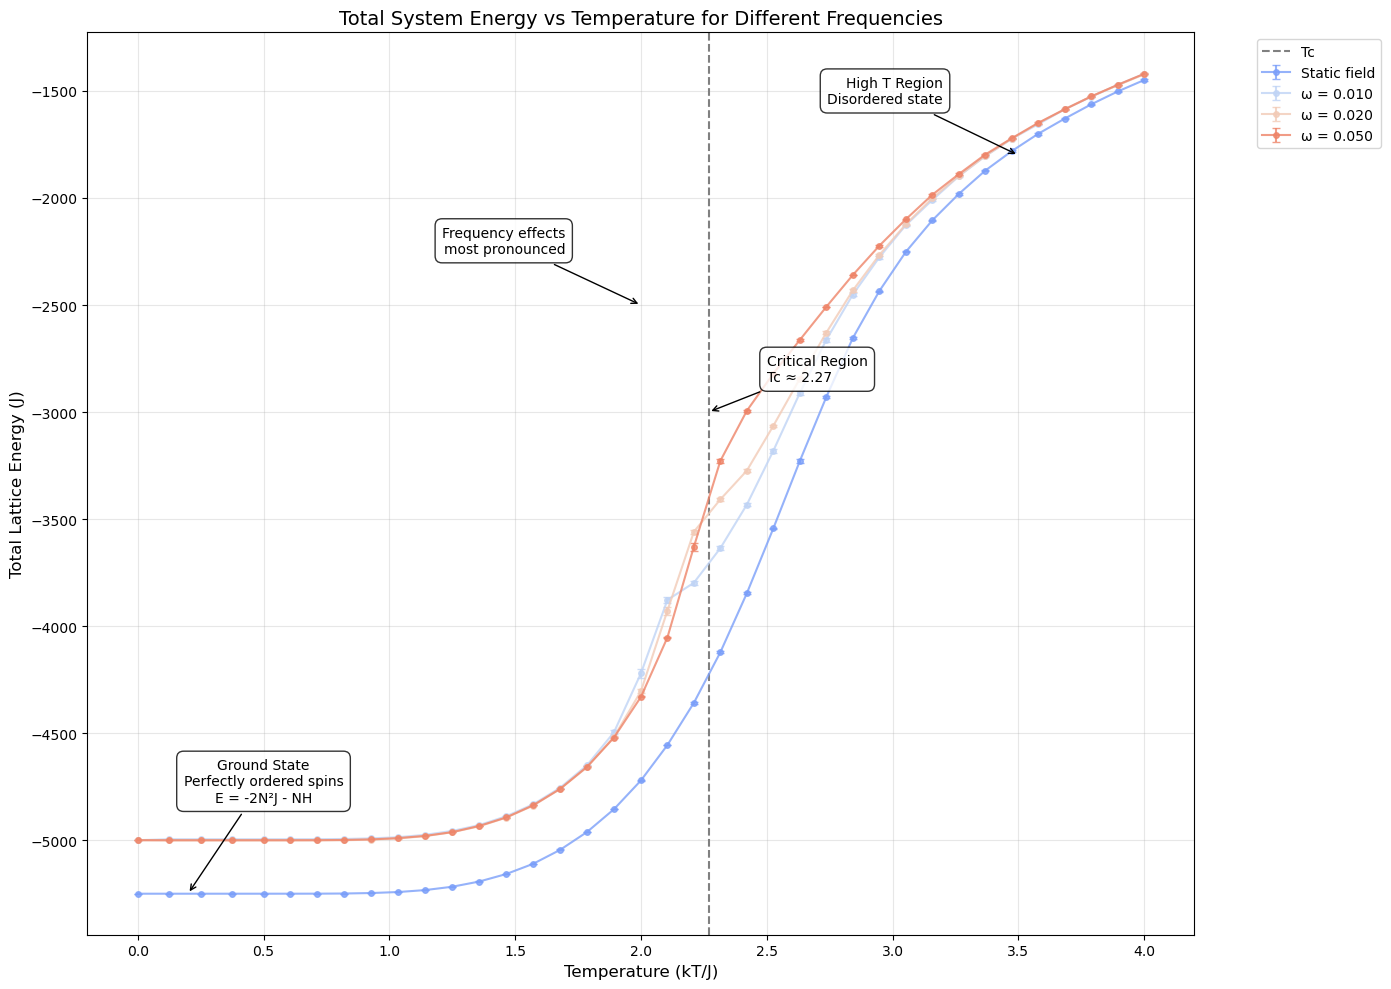
\includegraphics[width=\linewidth]{plots/heating E.png}
\caption{Total System Energy vs Temperature for different frequencies of the external field. The static field case shows the lowest energy state, while higher frequencies lead to higher system energies due to incomplete relaxation.}
\label{fig:energy}
\end{figure}

\subsection{Magnetization Behavior}

Figure~\ref{fig:magnetization} presents the normalized magnetization as a function of temperature, providing complementary insights into the phase transition. 

In the ordered phase ($T < T_c$), the magnetization remains fully aligned ($m = 1$) at $T = 0$ for all frequencies. However, the static field sustains the highest magnetization, while higher frequencies show an earlier departure from full alignment as temperature increases. 

In the critical region, the magnetization undergoes a sharp transition for the static field, whereas higher frequencies exhibit a broadening of this transition. Additionally, the effective critical temperature shifts depending on the frequency of the applied field. 

In the disordered phase ($T > T_c$), the magnetization converges to $m \approx 0$ for all frequencies. However, larger fluctuations are observed in systems subject to higher-frequency fields, indicative of increased dynamical effects.

\begin{figure}[h]
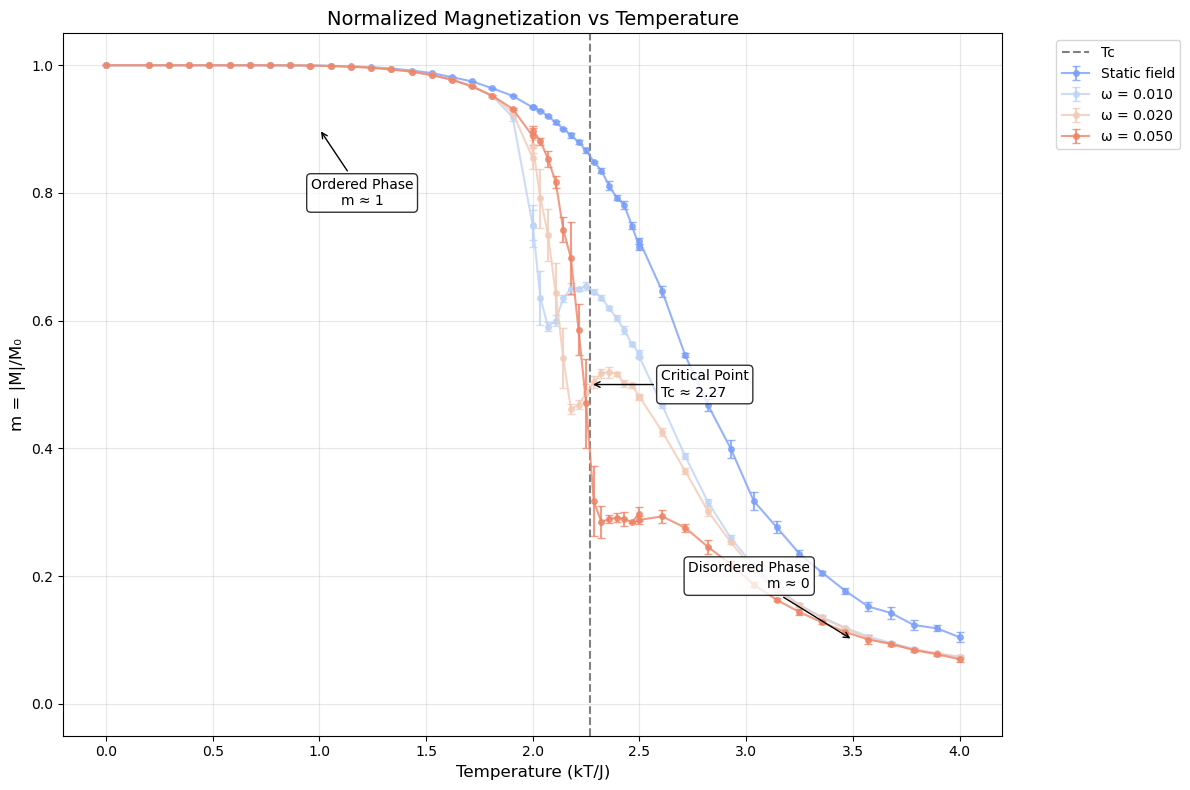
\includegraphics[width=\linewidth]{plots/heating M.png}
\caption{Normalized Magnetization vs Temperature showing the order-disorder transition. The effect of field frequency on the phase transition is clearly visible.}
\label{fig:magnetization}
\end{figure}

\subsection{Physical Interpretation}

These results reveal several important physical concepts. The system's response to an oscillating field is inherently frequency-dependent, showcasing the competition between the field's oscillation timescale and the system's natural relaxation time. 

Higher frequencies effectively reduce the field strength, as the system cannot keep pace with rapid oscillations. This phenomenon manifests in both the energy and magnetization behavior. Moreover, the oscillating field modifies the critical behavior of the phase transition, with higher frequencies leading to a more gradual transition between ordered and disordered states. 

These findings are consistent with theoretical predictions for dynamical effects in magnetic systems~\cite{Chakrabarti1999, Sides1998}.

\section{Code Implementation}

The numerical implementation employs a dynamic external field defined as:

\begin{verbatim}
H = H_amp * np.sin(omega * step) if omega > 0 else H_amp
\end{verbatim}

This implementation ensures proper time evolution of the external field, accurate energy calculation at each step, and correct handling of the $T=0$ case. Additionally, statistical averaging is performed over multiple field periods to ensure robust results.

\section{Acknowledgments}

For the simulation result and discussion. Xinyu is responsible for part 3.1 and appendix A. Tongzhou is responsible for part 3.2 and 3.3. Salar is responsible for part 4.



\bibliographystyle{unsrt}
\bibliography{refs}

\appendix
\section{A Hint on Proving the Metropolis Algorithm}\label{appendix}

The motivation lead to this appendix comes from the hardness to prove whether an ensemble is stabilized. Our target is to use metropolis algorithm to generate an ensemble $\mathcal{S}$ close to a true thermal ensemble $\mathcal{S_T}$, but it's hard to tell "the distance" between two ensemble. Although the convergence of metropolis algorithm to $\mathcal{S_T}$ can be proved theoretically, we would still like to give some additional hint on proving this. However, in this appendix, we cannot fully prove this point. We are only giving some hint to show that our $\mathcal{S}$ is close to $\mathcal{S_T}$.

We know that a thermal ensemble satisfies fluctuation-dissipation ensemble, which states that: at a fixed temperature $T$, the relative fluctuation of energy around expectation value$\frac{\sqrt{\langle \Delta E^2\rangle}}{\bar E}$ of an ensemble is inversely proportional to the heat capacity$C_V$ of the system:

\begin{equation}
    \sqrt{\langle \Delta E^2\rangle} \propto \frac{\bar E}{C_V}
\end{equation}

If our ensemble $\mathcal{S}$ generated by metropolis algorithm is close to a thermal ensemble, we should be able to observe this relation. We do simulation for our 2D Ising model with different size at fixed temperature $T'=3$ and calculated $\langle \Delta E^2\rangle$.\ref{fluctuation}

\begin{figure}
    \centering
    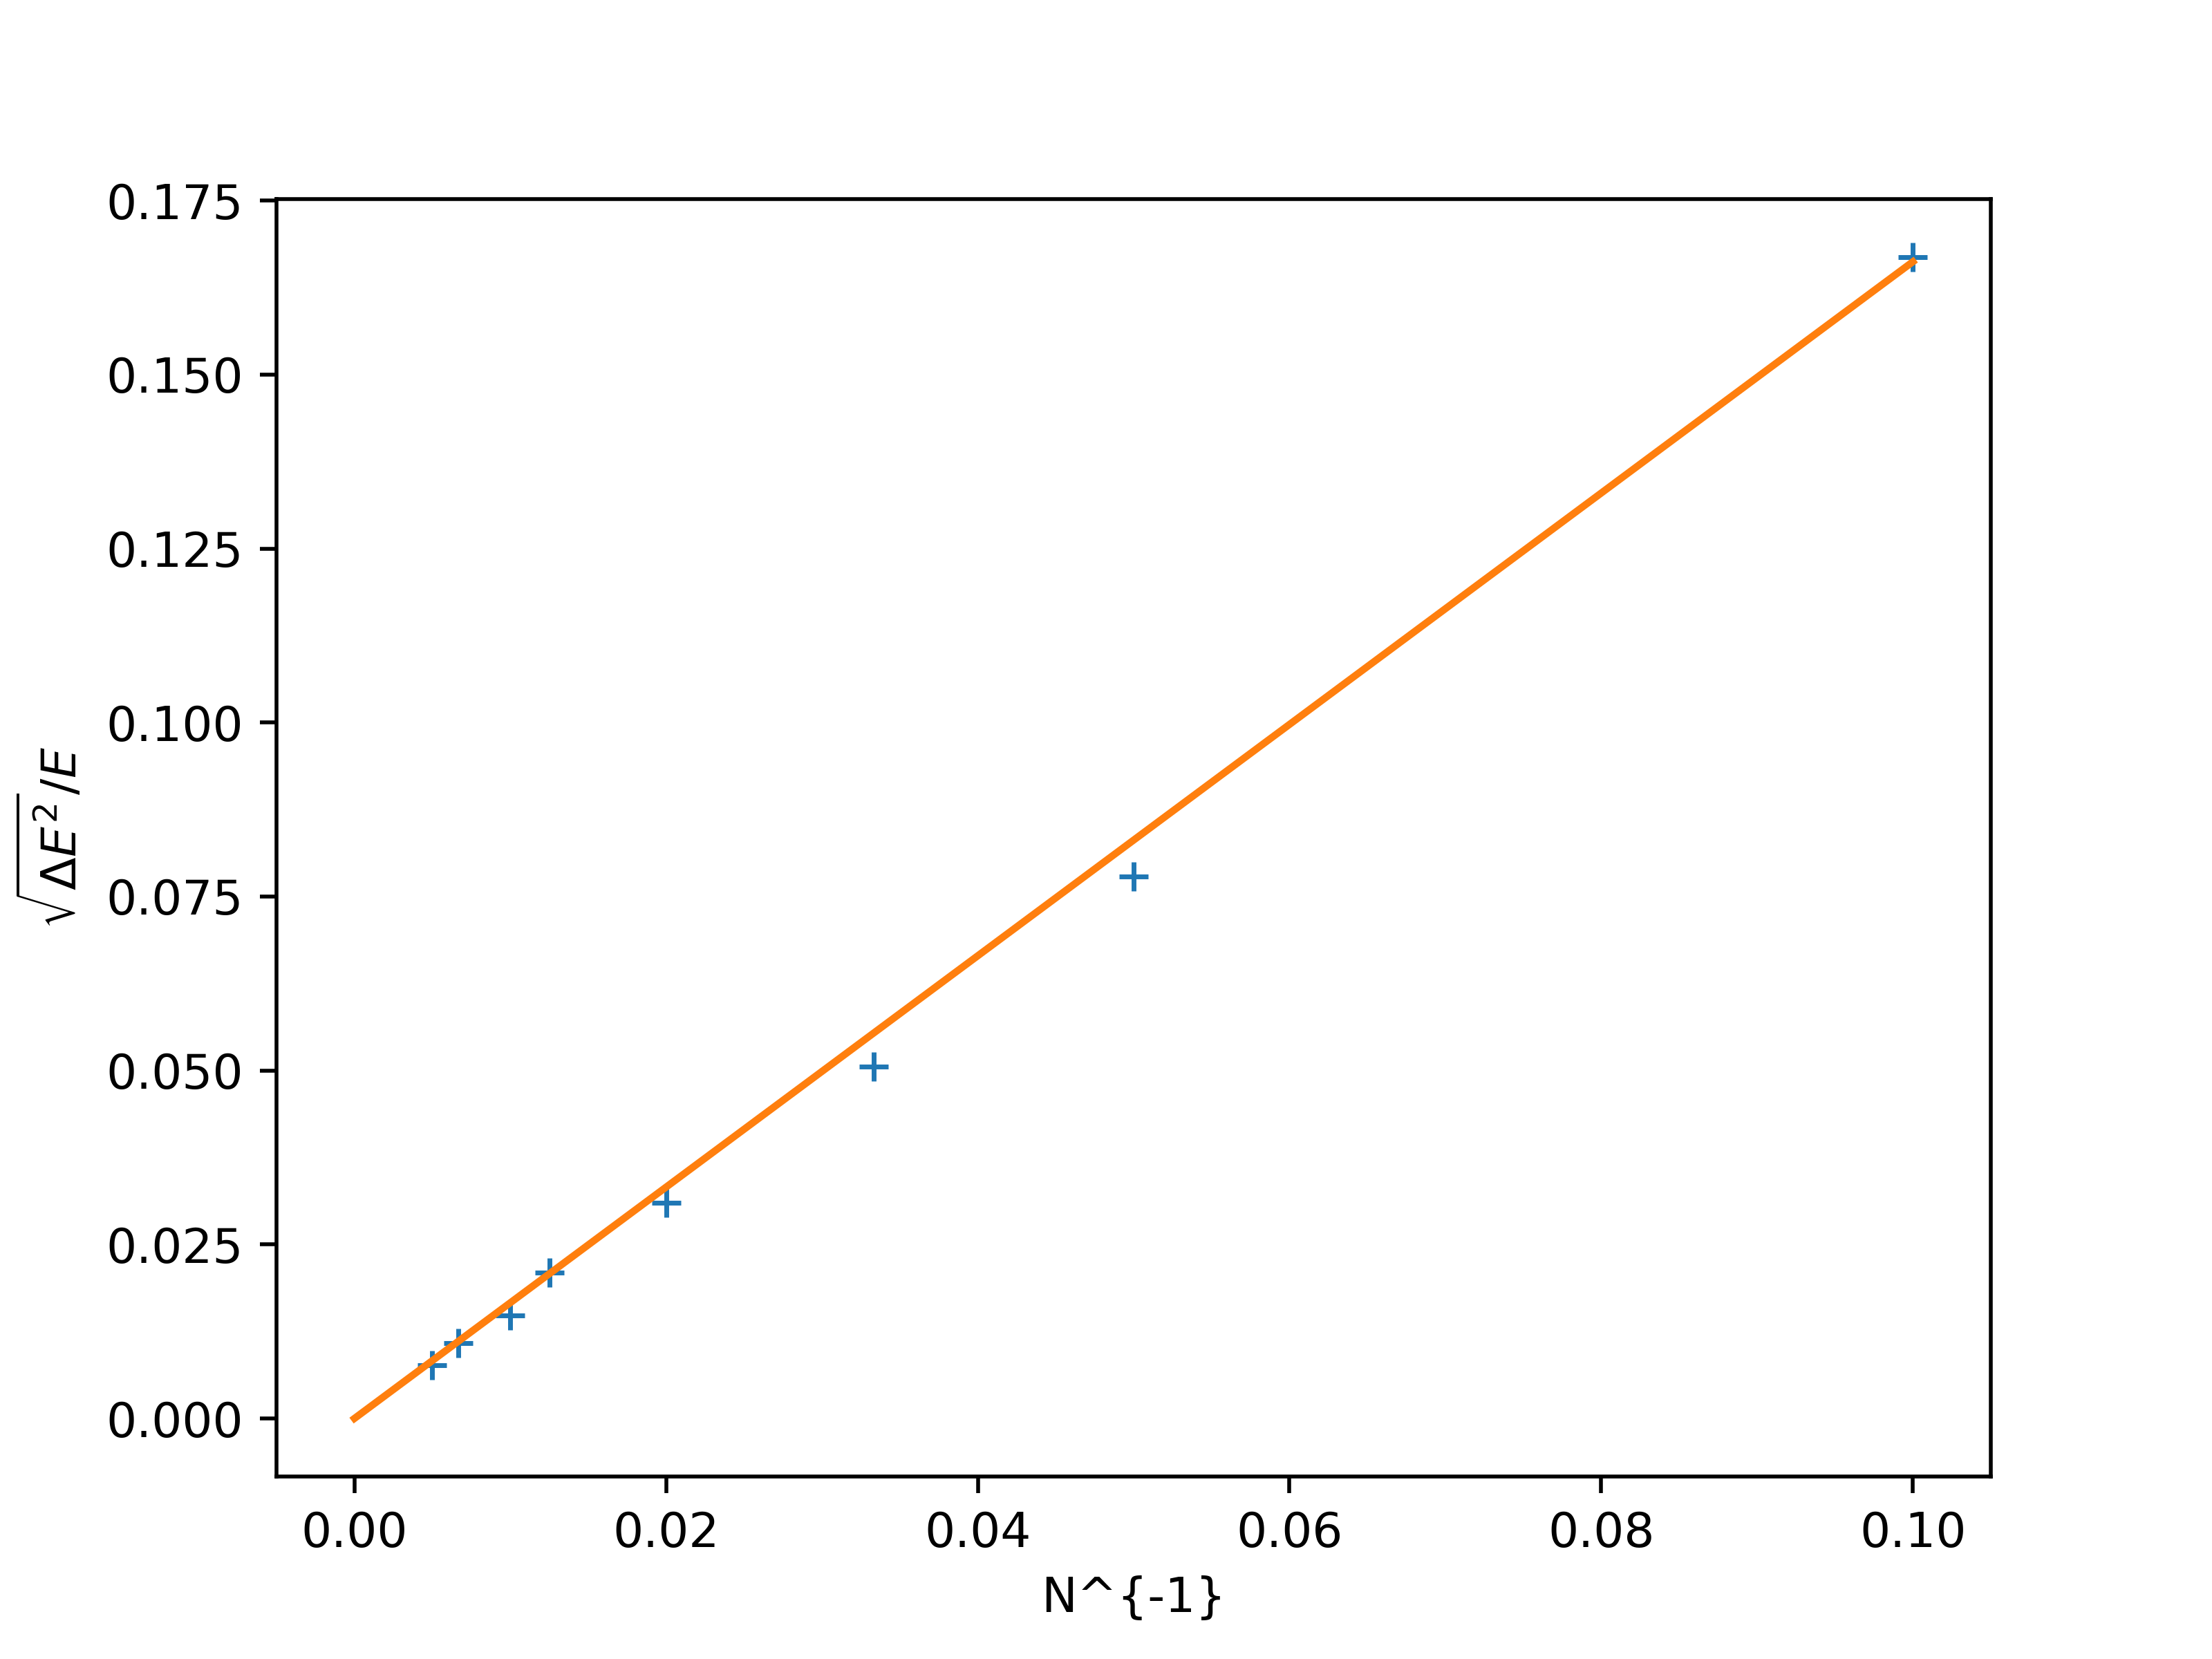
\includegraphics[width=0.8\linewidth]{plots/fluctuation-ensemblesize.png}
    \caption{Relative Energy Fluctuation of Our Model with Different Size $N$, at Temperature $T'=3$}
    \label{fluctuation}
\end{figure}

If the finite size effect is neglected, for a fixed temperature, the heat capacity $C_V$ is proportionally to the number of particle in the model:

\begin{equation}
    C_V \propto N^2
\end{equation}

In our data, we do can see that the relative energy fluctuation $\frac{\sqrt{\langle \Delta E^2\rangle}}{\bar E}$ is inversely proportionally the size $N$, after we do the linear regression, we find that:

\begin{equation}
    \frac{\sqrt{\langle \Delta E^2\rangle}}{\bar E} = 1.6622 * \frac{1}{N}  -0.0018
\end{equation}

With $r = 0.9991$. Note that we do not have a error bar on our diagram because we're already measuring the standard deviation of the energy. Although we have not perform simulation all possible cases, we do show that in this special case the fluctuation-dissipation theorem is satisfied by our ensemble $\mathcal{S}$. 


\end{document}
